\documentclass[11pt,a4paper]{article}

% ---------- language and type ----------
\usepackage{polyglossia}
\setdefaultlanguage[variant=british]{english}
\usepackage{fontspec}
\usepackage{unicode-math}
\setmainfont{EBGaramond}[
  Extension = .otf, UprightFont = *-Regular, ItalicFont = *-Italic,
  BoldFont = *-SemiBold, BoldItalicFont = *-SemiBoldItalic,
  Numbers = {Lining,Proportional}, Ligatures = TeX]
\setmonofont{Inconsolatazi4}[Extension = .otf, UprightFont = *-Regular, BoldFont = *-Bold, Scale = MatchLowercase, HyphenChar = None]
\setmathfont{Garamond-Math.otf}[StylisticSet={7,9,10}]
\newfontfamily\titleface{Cormorant Garamond SemiBold}[ItalicFont = {Cormorant Garamond Medium Italic}, Numbers = Lining, Ligatures = TeX]
\newfontfamily\ornfont{FreeSerif.otf}
\newfontfamily\qedface{EBGaramond}[Extension = .otf, UprightFont = *-Bold]
\newfontfamily\groupface{EBGaramond}[Extension = .otf, UprightFont = *-Medium, ItalicFont = *-MediumItalic, Numbers = {Lining,Proportional}]
\newfontfamily\labelface{EBGaramond}[Extension = .otf, UprightFont = *-Medium, Numbers = {Lining,Proportional}]
\newfontfamily\thmheadface{EBGaramond}[Extension = .otf, UprightFont = *-SemiBold]
\newcommand{\pagelabel}[1]{{\labelface\spacedsc{#1}}}
\newcommand{\spacedsc}[1]{{\scshape\addfontfeatures{LetterSpace=8}\MakeLowercase{#1}}}
\DeclareRobustCommand{\scn}[1]{{\upshape\addfontfeatures{Numbers={Lining,Proportional}}\scalebox{0.84}{#1}}}
\DeclareRobustCommand{\thd}[1]{{\scshape\addfontfeatures{LetterSpace=1.5}\MakeLowercase{#1}}}
\DeclareRobustCommand{\acr}[1]{{\addfontfeatures{Letters=UppercaseSmallCaps,LetterSpace=2}#1}}
\frenchspacing
\displaywidowpenalty=10000

% ---------- body size and leading: 11 on 14.6 ----------
\makeatletter
\renewcommand\normalsize{%
  \@setfontsize\normalsize{12}{15.2}%
  \abovedisplayskip 10\p@ \@plus2\p@ \@minus4\p@
  \abovedisplayshortskip 4\p@ \@plus3\p@
  \belowdisplayshortskip 7\p@ \@plus3\p@ \@minus3\p@
  \belowdisplayskip \abovedisplayskip
  \let\@listi\@listI}
\renewcommand\small{\@setfontsize\small{10.4}{13.4}}
\renewcommand\footnotesize{\@setfontsize\footnotesize{9.4}{12}}
\makeatother
\normalsize

% ---------- page ----------
\usepackage[a4paper,textwidth=132mm,top=33mm,bottom=39mm,headsep=9mm,footskip=14mm,headheight=14pt]{geometry}

\usepackage{amsmath,amsthm}
\usepackage{array}
\usepackage{tabularx}
\newcolumntype{L}[1]{>{\raggedright\arraybackslash}p{#1}}
\newcolumntype{Y}{>{\raggedright\arraybackslash}X}
\usepackage{booktabs}
\usepackage{longtable}
\setlength{\heavyrulewidth}{0.6pt}
\setlength{\lightrulewidth}{0.3pt}
\setlength{\extrarowheight}{2pt}
\usepackage{float}
\usepackage[section]{placeins}
\usepackage{xcolor}
\definecolor{oxford}{RGB}{0,33,71}
\definecolor{oxblood}{RGB}{116,30,44}
\definecolor{racing}{RGB}{24,74,52}
\usepackage{caption}
\DeclareCaptionLabelFormat{sclabel}{{\labelface\scshape\MakeLowercase{#1}}~{\labelface\scn{#2}}}
\captionsetup{figurename=Fig.,labelformat=sclabel,labelsep=period,margin=9mm,font=small,skip=7pt}
\usepackage{enumitem}
\setlist[enumerate]{label=(\roman*)}
\usepackage{etoolbox}

% ---------- headings: centred spaced small capitals; italic subheadings; no bold ----------
\usepackage{titlesec}
\usepackage{titletoc}
\setcounter{tocdepth}{1}
\titlecontents{section}[1.9em]{\small}{\contentslabel{1.9em}}{}{\hfill\contentspage}[\vspace{0.5pt}]
\titleformat{\section}[block]{\centering\titleface\fontsize{17pt}{20pt}\selectfont}{\thesection}{0.7em}{}
\titlespacing*{\section}{0pt}{30pt plus 5pt minus 3pt}{13pt}
\titleformat{\subsection}[block]{\normalsize\itshape}{\upshape\thesubsection}{0.75em}{}
\titlespacing*{\subsection}{0pt}{17pt plus 3pt minus 2pt}{6pt}
\titleformat{\subsubsection}[runin]{\normalsize\itshape}{\upshape\thesubsubsection}{0.6em}{}[.]
\titlespacing*{\subsubsection}{0pt}{9pt plus 2pt minus 1pt}{0.6em}

\usepackage{graphicx}
\usepackage{tikz}
\usetikzlibrary{positioning,arrows,calc,shadows}
\usepackage{pgfplots}
\pgfplotsset{compat=1.18}
\graphicspath{{./images/}}
\usepackage{lettrine}
\setcounter{DefaultLines}{2}
\renewcommand{\LettrineTextFont}{\scshape}

\widowpenalty=10000
\clubpenalty=10000
\usepackage{needspace}
\setlength{\intextsep}{11pt plus 3pt minus 2pt}
\setlength{\floatsep}{11pt plus 3pt minus 2pt}
\setlength{\textfloatsep}{16pt plus 4pt minus 2pt}
\makeatletter\setlength{\@fptop}{0pt}\setlength{\@fpsep}{18pt plus 4pt}\setlength{\@fpbot}{0pt plus 1fil}\makeatother
\renewcommand{\topfraction}{0.85}\renewcommand{\bottomfraction}{0.7}\renewcommand{\textfraction}{0.12}\renewcommand{\floatpagefraction}{0.75}

% ---------- tables: small, lining tabular figures ----------
\renewcommand{\arraystretch}{1.08}
\AtBeginEnvironment{tabular}{\footnotesize\addfontfeatures{Numbers={Lining,Tabular}}}
\AtBeginEnvironment{tabularx}{\footnotesize\addfontfeatures{Numbers={Lining,Tabular}}}

\usepackage{microtype}
\usepackage[superscript]{cite}

\makeatletter
\renewcommand\@biblabel[1]{#1.}
\renewenvironment{thebibliography}[1]
  {\section*{\refname}\small
   \list{\@biblabel{\@arabic\c@enumiv}}%
        {\settowidth\labelwidth{\@biblabel{#1}}%
         \leftmargin\labelwidth \advance\leftmargin\labelsep
         \setlength\itemsep{3.5pt plus 1pt}\setlength\parsep{0pt}%
         \usecounter{enumiv}\let\p@enumiv\@empty
         \renewcommand\theenumiv{\@arabic\c@enumiv}}%
   \sloppy\clubpenalty4000\widowpenalty4000\sfcode`\.\@m}
  {\def\@noitemerr{\@latex@warning{Empty `thebibliography' environment}}\endlist}
\makeatother

% ---------- abstract: centred small-capital label over an inset block ----------
\renewenvironment{abstract}{%
  \begin{center}{\footnotesize\pagelabel{Abstract}}\end{center}\vspace{-5pt}%
  \fontsize{10pt}{13.4pt}\selectfont
  \begin{list}{}{%
    \setlength{\leftmargin}{9mm}\setlength{\rightmargin}{9mm}%
    \setlength{\listparindent}{0pt}\setlength{\parsep}{6pt plus 2pt minus 1pt}%
    \setlength{\topsep}{0pt}\setlength{\partopsep}{0pt}%
  }\item[]\ignorespaces
}{\end{list}}

\usepackage{hyperref}
\pdfstringdefDisableCommands{\def\acr#1{#1}\def\spacedsc#1{#1}\def\thd#1{#1}\def\scn#1{#1}}
\hypersetup{
  colorlinks=true,
  allcolors=black,
  urlcolor=oxford,
  bookmarksnumbered=true,
  bookmarksopen=true,
  bookmarksopenlevel=1,
  pdfdisplaydoctitle=true,
  pdflang=en-GB,
  pdfauthor={K.R. Ryan},
  pdftitle={The Geometric Siphon: Existence, Equilibrium, and Directional Properties of the Residual in Concentrated Liquidity Portfolios},
  pdfsubject={Concentrated liquidity, geometric residual, directional and exit asymmetries},
  pdfkeywords={geometric residual, directional asymmetry, exit asymmetry, automated market maker, Uniswap V3, Aerodrome, DeFi mechanism design}
}
\PassOptionsToPackage{hyphens}{url}
\Urlmuskip=0mu plus 1mu
\urlstyle{same}
\def\UrlBreakPenalty{10000}
\def\UrlBigBreakPenalty{10000}
\usepackage[bottom]{footmisc}
\renewcommand{\footnotelayout}{\fontsize{8.6pt}{11.4pt}\selectfont}
\setlength{\footnotesep}{9pt}
\setlength{\skip\footins}{16pt plus 4pt minus 2pt}

% ---------- running head: spaced small capitals, centred; folio at the foot ----------
\usepackage{fancyhdr}
\pagestyle{fancy}
\fancyhf{}
\fancyhead[C]{\footnotesize\spacedsc{The Geometric Siphon}}
\fancyfoot[C]{\small\thepage}
\renewcommand{\headrulewidth}{0pt}
\fancypagestyle{plain}{\fancyhf{}\fancyfoot[C]{\small\thepage}\renewcommand{\headrulewidth}{0pt}}

% ---------- theorems: small-capital label, name in roman, statement in italic ----------
\newtheoremstyle{siphon}{11pt plus 2pt minus 1pt}{10pt plus 2pt minus 1pt}{\itshape}{}{}{}{\newline}%
  {{\thmheadface\scshape\MakeLowercase{\thmname{#1}}\thmnumber{ \scn{#2}}}\thmnote{\upshape\enspace\textperiodcentered\enspace #3}\vadjust{\vskip 3pt}}
\theoremstyle{siphon}
\newtheorem{theorem}{Theorem}
\newtheorem{corollary}{Corollary}[theorem]
\newtheorem{conjecture}{Conjecture}
\renewcommand{\thetheorem}{\arabic{theorem}}
\renewcommand\qedsymbol{\raisebox{0.17ex}{\scalebox{0.68}{\ensuremath{\mdlgblksquare}}}}

\usepackage{mdframed}
\newenvironment{codeblock}{%
  \begin{mdframed}[%
    backgroundcolor=white,%
    linewidth=0.5pt,linecolor=black!30,topline=false,bottomline=false,rightline=false,%
    innertopmargin=6pt,%
    innerbottommargin=6pt,%
    innerleftmargin=12pt,%
    innerrightmargin=12pt,%
    leftmargin=1.25em,%
    rightmargin=0pt,%
    skipabove=6pt,%
    skipbelow=6pt%
  ]\footnotesize%
}{%
  \end{mdframed}%
}

\setlength{\parindent}{1.25em}
\setlength{\parskip}{0pt}
\tolerance=1400
\emergencystretch=1.5em

\newtheorem{proposition}[theorem]{Proposition}

\begin{document}
\thispagestyle{plain}

\begin{center}
\vspace*{11mm}
{\fontsize{32pt}{37pt}\selectfont\titleface The Geometric Siphon}\\[12pt]
{\fontsize{15.5pt}{20pt}\selectfont\titleface\itshape Existence, Equilibrium, and Directional Properties\\
of the Residual in Concentrated Liquidity Portfolios}\\[19pt]
\rule{16mm}{0.4pt}\\[15pt]
{\fontsize{12pt}{14pt}\selectfont\spacedsc{K.\,R. Ryan}}\\[7pt]
{\fontsize{9pt}{12pt}\selectfont\itshape April 2026, revised November 2026}
\end{center}
\vspace{-5pt}
\centerline{\scalebox{1.15}{$\therefore$}}
\vspace{7pt}

\begingroup\renewcommand\thefootnote{}\footnotetext{\hypersetup{allcolors=black}Independent researcher \enspace\textperiodcentered\enspace {\scshape orcid}\enspace{\addfontfeatures{Numbers={OldStyle,Proportional}}\href{https://orcid.org/0009-0004-6295-7040}{0009-0004-6295-7040}} \enspace\textperiodcentered\enspace \href{mailto:gancor@gancor.xyz}{gancor@gancor.xyz}}\endgroup
\begingroup\renewcommand\thefootnote{}\footnotetext{This version revises that of May 2026. Its empirical sections are rebuilt from on-chain events (Appendix~\ref{app:changes}).}\endgroup

\begin{abstract}
This paper identifies and formalises the \emph{Geometric Siphon}, a mechanism that arises from the geometry of concentrated liquidity rebalancing and becomes observable when positions share a depositor balance. A rebalance that changes the required token ratio leaves a residual, and a shared balance lets positions in other pools redeploy it, which transfers capital between them. Six theorems give the residual in closed form with the condition under which it vanishes, convergence in expectation for same-pool positions, geometric extinction without a swap, and monotonicity, directional, and exit asymmetries in a stated unit of account. Six propositions follow the residual through the position manager's internal swap into the shared balance and give an accounting rule that removes the transfer. The theorem layer is largely formalised in Lean and checked in a Foundry suite, in part against unmodified Slipstream contracts. On about $280{,}000$ production rebalances over seven months, the residual on unchanged ranges is a median $10^{-11}$ of position value, and the transfer redistributed a net \$121{,}500 among positions, zero-sum within each shared balance, leaving a position's realised return almost uncorrelated with its own (rank correlation $0.02$ across 107 positions).
\end{abstract}

\begin{center}
\fontsize{9pt}{12.5pt}\selectfont
\pagelabel{Keywords}\enspace geometric residual \textperiodcentered\ directional asymmetry \textperiodcentered\ automated market maker\\
Uniswap V3 \textperiodcentered\ Aerodrome \textperiodcentered\ DeFi mechanism design\\[2pt]
\pagelabel{\acr{JEL}}\enspace G12, G14, G19, G23
\end{center}

\vspace{12pt}
\begin{center}
\begin{minipage}{84mm}
\centerline{\footnotesize\pagelabel{Contents}}\vspace{5pt}
\makeatletter\@starttoc{toc}\makeatother
\end{minipage}
\end{center}
\vspace{6pt}

\section{Introduction}\label{sec:introduction}

\lettrine[findent=2pt,nindent=0pt]{C}{oncentrated liquidity}, introduced in Uniswap V3,\cite{adams2021} requires active management. Every major \acr{CL} automation platform (Gamma Strategies, Arrakis Finance, Beefy \acr{CLM}) uses a \emph{vault-per-pool} architecture in which one vault manages one token pair and leftover tokens from rebalances are reinvested into the same position. Residuals stay in the pool that produced them and appear, if at all, as a small capital efficiency loss difficult to separate from slippage.

Position Manager V6 (\acr{PMV}\scn{6}), a \acr{CL} management contract on Base, accounts for residuals differently. Leftover tokens have no pool dimension and are held in \texttt{dustBalance[depositor][token]}, keyed by depositor and token only (Appendix~\ref{app:contract}), so every position under one depositor draws from the same balance. That accounting choice opens a channel through which residuals from one pool can be absorbed by positions in another. This paper characterises that channel and the residual that drives it.

On 2 March 2026, routine monitoring of one such \acr{PMV}\scn{6} deployment revealed that a \acr{USDC}/\acr{CHECK} position had grown about $65\%$ while a \acr{USDC}/\acr{ODOS} position in the same depositor group had shrunk about $60\%$, although \acr{USDC} was their only shared token. \acr{CHECK} was consuming \acr{USDC} residuals left behind by \acr{ODOS} rebalances through the shared dust pool. The initial assumption was slippage; an on-chain decomposition of 92 rebalance transactions instead showed that slippage accounted for only a small part of the transfers, which pointed to the geometric mismatch between consecutive tick ranges. I call this mechanism the \emph{Geometric Siphon}.

Cross-pool flow requires only that residuals be accessible through a shared balance across positions that keeps no per-position account of them. This design choice is unusual in current production but not unique to \acr{PMV}\scn{6}, and any protocol that adopts it inherits the mechanism.

The discovery raises three questions: when does the residual vanish, what governs the long-run behaviour of positions exposed to it, and how does its \acr{USD}-denominated value respond to price direction and exit type? Section~\ref{sec:theory} answers them in six theorems. Two further questions follow, namely what the position manager's internal swap leaves behind and which position ends up holding it, and six propositions answer them (\S\S\ref{sec:leftover}--\ref{sec:ownership}). The \emph{residual} is the ratio mismatch of a range change and is a property of the geometry alone. The \emph{leftover} is the part of the residual that the internal swap does not absorb and that enters the shared dust pool. The \emph{transfer} is the part of a mint above the position's own equity, which is leftover from other positions (\S\ref{sec:ownership}). A 16-test Foundry suite verifies Theorems~\ref{thm:residual} and~\ref{thm:extinction}--\ref{thm:exit}, six of its tests running as live fork tests against unmodified V3 contracts on Aerodrome Slipstream. A \acr{USDC}/\acr{ZARP} trajectory ($\$942$ to $\$1.59$ in 14 rebalances) illustrates the zero-swap loss of Theorem~\ref{thm:residual} on its two zero-swap events, and the partial-swap decay of Proposition~\ref{prop:partial} on most of the rest.

Two bodies of evidence anchor the empirical results. A 1{,}380-event controlled phase spanning 39 positions over 7 days is consistent with the existence claim and contains both a single realisation of single-pool convergence and a partial-swap extinction trajectory. An on-chain dataset for the same contract family, rebuilt from pool and contract events (\S\ref{sec:record}), supplies the measurements at scale. It holds approximately $280{,}000$ rebalances of the \acr{PMV}\scn{9} deployment between 21~March and 14~October 2026, and about $26{,}400$ rebalances of \acr{PMV}\scn{6}--\acr{PMV}\scn{8} on which a prediction specified in advance is tested.

Section~\ref{sec:related} places the paper in the V3 \acr{LP} economics literature. The theoretical results and their main proof ideas follow next, with fuller derivations collected in Appendix~\ref{app:dr-derivation}. Section~\ref{sec:experimental} describes the Phase~1--3 design, and Section~\ref{sec:results} reports the results. Section~\ref{sec:foundry} summarises the Foundry verification, detailed in Appendix~\ref{app:foundry-detailed}. Section~\ref{sec:discussion} discusses the architectural precondition, the unit-of-account question, and the limitations. Section~\ref{sec:conclusion} concludes.

\section{Related work}\label{sec:related}

Concentrated liquidity in Uniswap V3\cite{adams2021} supplies the amount equations from which all six theorems derive.

Three lines of theoretical work model costs incurred by V3 \acr{LP}s between rebalances. Hasbrouck et al.\cite{hasbrouck2025} model \acr{CL} provision as a covered call sold at intrinsic rather than market value, so \acr{LP}s forgo the option's time premium in exchange for fees; equilibrium liquidity provision decreases as that time premium rises. Cartea et al.\cite{cartea2024} introduce \emph{predictable loss}, a closed-form measure of unhedgeable losses comprising convexity loss from informed trading and opportunity cost on locked capital, and analyse \emph{concentration risk}, the decrease in fee revenue when the marginal exchange rate exits the \acr{LP}'s range of liquidity. Milionis et al.\cite{milionis2022b} introduce \acr{LVR} (Loss-Versus-Rebalancing), the return gap between an \acr{AMM} \acr{LP} and a continuously rebalancing benchmark driven by arbitrage against stale \acr{AMM} prices. Milionis et al.\cite{milionis2024} extend the framework to fees and discrete block timing.

The geometric residual studied here is distinct from those loss mechanisms. It arises at the rebalance itself, is determined by the geometry of $R(s, s_a, s_b)$ rather than by price trajectory, exposure, or arbitrage, and is zero on same range rebalances regardless of price travel (Theorem~\ref{thm:residual}). The Phase~1 decomposition separates observed dust flow from swap slippage (\S\ref{sec:decomposition}), and the on-chain dataset identifies the residual generated by range changes (\S\ref{sec:ledger}). Theorems~\ref{thm:directional} and~\ref{thm:exit} identify \acr{USD}-denominated asymmetries that are mechanistically separate from, but parallel in form to, the option-theoretic asymmetry of Hasbrouck et al.\cite{hasbrouck2025} and the boundary-event behaviour analysed by Cartea et al.\cite{cartea2024}.

Empirical work on V3 \acr{LP}s has focused on per-position risk and return distributions. Heimbach et al.\cite{heimbach2022} find wide cross-strategy variation that rewards active management. Loesch et al.\cite{loesch2021} find that about half of the liquidity providers in 17 large V3 pools earned less in fees than they lost to impermanent loss over May to September 2021. Willetts and Harrington\cite{willetts2026} measure arbitrage efficiency and rebalancing costs in dynamic-weight \acr{AMM} pools on Ethereum and Base under \acr{LVR} benchmarks, the closest published empirical context for per-rebalance cost analysis on Base L2. The empirical results below extend this line of work to an on-chain dataset of approximately $280{,}000$ rebalances focused on rebalance-event dust flows.

Fan et al.\cite{fan2023} formulate the \acr{LP}'s strategic problem as choosing tick ranges to maximise fees net of repositioning costs, treating each position in isolation. Theorems~\ref{thm:monotonicity}--\ref{thm:exit} characterise the asymmetries that any such strategy faces under directional price moves and at range exits.

Several alternative rebalancing architectures exist at the protocol level. Balancer\cite{martinelli2019} rebalances via its \acr{AMM} invariant within a single pool; Set Protocol uses oracle-triggered swaps; Yearn deploys capital across strategist-managed strategies. All require a shared pool invariant, external price feeds, or manual intervention. Maverick Protocol's directional liquidity modes\cite{maverick2023} have bins follow price automatically; `Mode Both' is the closest analogue to siphon-driven repositioning, being continuous, automatic, and oracle-free, but operates within a single position. The Geometric Siphon arises from \acr{CL} geometry alone and operates across positions in different pools, requiring only a depositor-level shared dust balance.

Geometric residual flows between \acr{CL} positions sharing depositor-level balances do not appear in the literature surveyed here. Nor do the directional and exit asymmetries of those residuals (Theorems~\ref{thm:directional}, \ref{thm:exit}), which follow from the same V3 amount equations.

A concurrent \acr{SSRN} preprint by I.\,P.\cite{secondoperator2026} develops a graph-theoretic treatment of the same mechanism on a port of the present author's Position Manager to Uniswap V3. Its results are compatible with those here, including a residual-generation lemma equivalent to Theorem~\ref{thm:residual}, a circulation-path condition for cross-pool absorption (token degree $\geq 2$ in the portfolio graph), and a directional-convexity scaling for symmetric price displacements.

\section{Theoretical framework}\label{sec:theory}

Taken together, the results in this section proceed from existence to dynamics to asymmetry. Theorem~\ref{thm:residual} identifies when a rebalance does and does not generate a geometric residual, separating geometry-driven flow from slippage and motivating the decomposition tested in \S\ref{sec:decomposition}. Theorems~\ref{thm:convergence} and~\ref{thm:extinction} then characterise opposite dynamical regimes of the same mechanism, with Theorem~\ref{thm:convergence} giving expected same-pool convergence under shared balances and Theorem~\ref{thm:extinction} giving geometric extinction under repeated zero-swap rebalancing. Theorems~\ref{thm:monotonicity}--\ref{thm:exit} turn to displacement, direction, and exit type, showing how residual magnitude and retained \acr{USD} value vary once a stablecoin num\'eraire is fixed. Sections~\ref{sec:leftover}--\ref{sec:ownership} then follow the residual through the internal swap and into the shared dust pool. Readers primarily interested in the empirical results may treat this section as a guide to the formal claims; full derivations of the six theorems are in Appendix~\ref{app:dr-derivation}.

\subsection{Concentrated liquidity preliminaries}\label{sec:preliminaries}

The results below rely on the standard Uniswap V3 amount equations, the token ratio implied by a range at the current price, and the corresponding position value in token1 units.

\medskip
\noindent\emph{Token amounts in the position.}
\begin{equation}\label{eq:amounts}
x = L\biggl(\frac{1}{s} - \frac{1}{s_b}\biggr),
\qquad
y = L (s - s_a).
\end{equation}

\noindent\emph{Ratio of the two token amounts.}
\begin{equation}\label{eq:ratio}
R(s, s_a, s_b) = \frac{x}{y} = \frac{1/s - 1/s_b}{s - s_a}.
\end{equation}

\noindent\emph{Position value, in token1 units.}
\begin{equation}\label{eq:value}
V = x s^2 + y = L\phi(s, s_a, s_b),
\qquad
\phi(s, s_a, s_b) = 2s - \frac{s^2}{s_b} - s_a.
\end{equation}

\textit{Notation.} The symbols used throughout the paper are summarised in Table~\ref{tab:notation} in Appendix~\ref{app:dr-derivation}.

\subsection{The geometric residual}\label{sec:residual}

A rebalance withdraws liquidity from $[s_a, s_b]$ and mints into $[s_a', s_b']$ at the same current price $s$. By~\eqref{eq:amounts} and~\eqref{eq:ratio} the withdrawn amounts $(x_w, y_w)$ are in the ratio $R_{\symup{old}} = R(s, s_a, s_b)$, and the new range requires the ratio $R_{\symup{new}} = R(s, s_a', s_b')$.

The new liquidity is determined by the per-token minimum,
\begin{equation}\label{eq:lnew-min}
L_{\symup{new}} = \min\biggl(\frac{x_w}{1/s - 1/s_b'}, \; \frac{y_w}{s - s_a'}\biggr),
\end{equation}
with the token1 term binding when $R_{\symup{old}} \geq R_{\symup{new}}$ (excess token0) and the token0 term binding when $R_{\symup{old}} < R_{\symup{new}}$ (excess token1). The binding token is the \emph{missing token} of the rebalance and the other is the \emph{surplus token}, left in strict excess whenever $R_{\symup{old}} \neq R_{\symup{new}}$.

Consider the isolated case, in which no shared balance tokens contribute to the mint and no swap is made. Write $V = V_{\symup{old}}$ for the pre-rebalance value, $V_{\symup{new}} = L_{\symup{new}}\,\phi(s, s_a', s_b')$ for the value minted, and $\Delta R = V_{\symup{new}} - V_{\symup{old}}$ for the signed residual value of the rebalance. In a shared balance setting, $D$ is the observed event-level dust flow and $D_{\symup{pool}}$ the accumulated stock of contract dust available for absorption; $D/V$ can have either sign, depending on whether the mint absorbs surplus from $D_{\symup{pool}}$ or contributes to it.

By~\eqref{eq:ratio} and~\eqref{eq:value}, a position whose amounts are in the ratio $R$ holds the fractions
\begin{equation}\label{eq:fractions}
\frac{R s^2}{1 + R s^2} \quad\text{and}\quad \frac{1}{1 + R s^2}
\end{equation}
of its value in token0 and token1. Let $\omega$ be the fraction of the withdrawn value held in the missing token and $\omega'$ the fraction of a position's value that the new range requires in the same token. These are~\eqref{eq:fractions} at $R = R_{\symup{old}}$ and at $R = R_{\symup{new}}$.

\needspace{4\baselineskip}
\begin{theorem}[Geometric residual]\label{thm:residual}
For a concentrated liquidity rebalance from range $[s_a, s_b]$ to $[s_a', s_b']$ at current sqrt price $s$, with $s$ in the interior of both ranges, the residual in the isolated case is
\begin{equation}\label{eq:share}
\frac{\Delta R}{V} = -\,\frac{\omega' - \omega}{\omega'} \leq 0,
\end{equation}
where $\omega$ and $\omega'$ are the fractions of value in the missing token, as withdrawn and as the new range requires. Equality holds if and only if $R(s, s_a, s_b) = R(s, s_a', s_b')$.
\end{theorem}

\noindent The rebalance has zero residual value if and only if the old and new ranges require the same token ratio at the current price. Otherwise the residual is the shortfall of the missing token, $\omega' - \omega$, as a fraction of what the new range requires of it. The companion paper on rebalancing cost states the same quantity in logarithmic form.\cite{ryan2026localtime}

\begin{proof}\renewcommand\qedsymbol{\smash{{\normalfont\qedface\fontsize{12.5pt}{12.5pt}\selectfont\scshape\addfontfeatures{LetterSpace=7}q.e.d.}}}
By~\eqref{eq:ratio}, the token1 term of~\eqref{eq:lnew-min} is the smaller exactly when $R_{\symup{old}} \geq R_{\symup{new}}$. The mint takes all of the missing token, an amount worth $\omega V$, and that token makes up the fraction $\omega'$ of the new position's value. Hence
\[
\omega'\,V_{\symup{new}} = \omega\,V ,
\]
which is the equality in~\eqref{eq:share}. Of the fractions~\eqref{eq:fractions}, that of token1 is strictly decreasing in $R$ and that of token0 strictly increasing. Token1 is missing when $R_{\symup{old}} \geq R_{\symup{new}}$ and token0 when $R_{\symup{old}} < R_{\symup{new}}$, so in either case $\omega \leq \omega'$, with equality exactly when $R_{\symup{old}} = R_{\symup{new}}$. The withdrawn amounts then already match the ratio required by the new range and both tokens redeploy in full.
\end{proof}
\vspace{9pt}

\needspace{4\baselineskip}
\begin{corollary}[Ratio-preserving ranges]\label{cor:locus}
At fixed $s$, the new ranges with zero residual are those satisfying
\[
\frac{1}{s_b'} = \frac{1}{s} - R_{\symup{old}}\,(s - s_a') .
\]
This is one equation in two unknowns and therefore defines a one-dimensional curve in the $(s_a', s_b')$ plane, with one upper bound for each admissible lower bound. The original range $(s_a, s_b)$ lies on that curve, but does not exhaust it. Range equality is thus sufficient for a zero residual but not necessary.
\end{corollary}

\noindent A ratio-preserving range leaves the composition of the position as it was, so no such range recentres a displaced position.

\needspace{4\baselineskip}
\begin{corollary}[Round trip]\label{cor:roundtrip}
Let two ranges containing $s$ require the fractions $\omega_A \leq \omega_B$ of value in token0. In the isolated case, a rebalance from one to the other and back at the price $s$ leaves the fraction
\[
\frac{\omega_A\,(1 - \omega_B)}{\omega_B\,(1 - \omega_A)}
\]
of the position's value deployed, whichever range it starts from.
\end{corollary}

\noindent Token0 is missing on the step from $A$ to $B$ and token1 on the step back, and~\eqref{eq:share} applies to each. The fraction is the ratio of the odds of the two compositions. It is below one unless the ranges are ratio-preserving, so reversing a range change does not recover its residual. The companion paper develops the single step as a cost potential.\cite{ryan2026localtime}

\subsection{Two-mechanism structure}\label{sec:two-mechanism}

Theorem~\ref{thm:residual} partitions rebalances into ratio-changing events ($\Delta R \neq 0$) and ratio-preserving events ($\Delta R = 0$). On chain, about half of all rebalances are ratio-changing (\S\ref{sec:two-mechanism-split}). Same-range events nonetheless produce non-zero $|D|$, which only a contract-level dust pool can explain.

\textit{Stage~1: Geometric creation.} Range-change rebalances produce geometric residuals via~\eqref{eq:lnew-min}. The position manager's internal swap absorbs between $98\%$ and $99.7\%$ of the ratio mismatch (\S\ref{sec:ledger}); the remainder enters the shared dust pool as unmatched tokens. This remainder, the dust that one rebalance adds to the pool, is called the \emph{leftover} below, and \S\ref{sec:leftover} gives its size and its token. Without range changes, the pool is no longer replenished and drains towards zero.

\textit{Stage~2: Dust-pool redistribution.} Rebalances draw from accumulated contract dust. The \acr{CL} mint function uses all available tokens,
\begin{equation}\label{eq:mint}
L_{\symup{new}} = \min\biggl(\frac{x_w + x_{\symup{dust}}}{1/s - 1/s_b'}, \; \frac{y_w + y_{\symup{dust}}}{s - s_a'}\biggr),
\end{equation}
so excess pool dust on the non-binding side is absorbed ($D > 0$), while an imbalance in the withdrawn amounts leaves residual dust ($D < 0$). The observed dust flow $D$ of an event is therefore what the position absorbs from the dust pool less the leftover it adds, apart from the cost of the swap. Dust that a position absorbs and another position left is a \emph{transfer} between the two, defined exactly in \S\ref{sec:ownership}.

Fig.~\ref{fig:mechanism} traces one rebalance through both stages.

\begin{figure}[!htb]
\vspace{2pt}
\centering
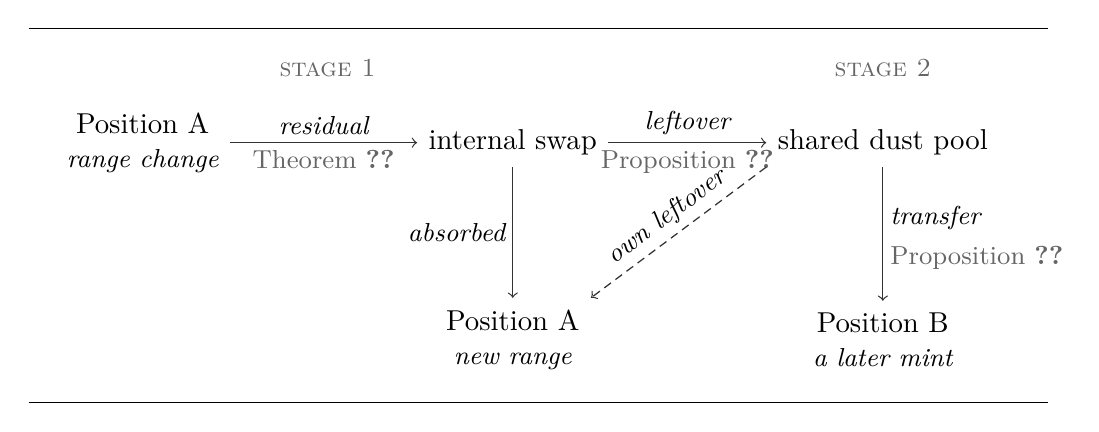
\begin{tikzpicture}[
  >=to,
  font=\small,
  obj/.style  = {align=center, inner sep=4pt},
  lab/.style  = {font=\footnotesize\itshape, inner sep=2.5pt},
  src/.style  = {font=\footnotesize, text=black!60, inner sep=2.5pt},
  flow/.style = {->, draw=black!80, line width=0.45pt},
]
\draw[line width=0.6pt] (-1.45,1.45) -- (11.5,1.45);
\node[obj] (a)  at (0,0)       {Position A\\[-1pt]{\footnotesize\itshape range change}};
\node[obj] (s)  at (4.7,0)     {internal swap};
\node[obj] (d)  at (9.4,0)     {shared dust pool};
\node[obj] (a2) at (4.7,-2.5)  {Position A\\[-1pt]{\footnotesize\itshape new range}};
\node[obj] (b)  at (9.4,-2.5)  {Position B\\[-1pt]{\footnotesize\itshape a later mint}};
\draw[flow] (a) -- node[lab, above] {residual} node[src, below] {Theorem~\ref{thm:residual}} (s);
\draw[flow] (s) -- node[lab, above] {leftover} node[src, below] {Proposition~\ref{prop:leftover}} (d);
\draw[flow] (s) -- node[lab, left] {absorbed} (a2);
\draw[flow] (d) -- node[lab, right, pos=0.38] {transfer} node[src, right, pos=0.68] {Proposition~\ref{prop:neutral}} (b);
\draw[flow, densely dashed] (d.south west) -- node[lab, sloped, above] {own leftover} (a2.north east);
\node[src] at (2.35,0.95) {\textsc{stage 1}};
\node[src] at (9.4,0.95)  {\textsc{stage 2}};
\draw[line width=0.6pt] (-1.45,-3.3) -- (11.5,-3.3);
\end{tikzpicture}
\caption{The siphon mechanism.}
\label{fig:mechanism}
\vspace{2pt}
\end{figure}

The siphon requires all three components. Removing any one shuts the mechanism off in a different way, and each removal is observed in \S\ref{sec:results}.

In steady state, the two flows balance. Same range rebalances create no residual and can only absorb from the dust pool, while range changes both add the leftover and absorb what earlier events left (\S\ref{sec:two-mechanism-split}).

\begin{table}[H]
\centering
\caption{The three components, and what happens without each.}
\label{tab:siphon-components}
\renewcommand{\arraystretch}{1.15}
\begin{tabular}{@{}lL{7.6cm}l@{}}
\toprule
\thd{Component} & \thd{Without it} & \thd{Shown in}  \\
\midrule
Range changes & No residual is created, and the dust pool is not replenished & \S\ref{sec:ledger} \\
A leftover after the swap & Nothing enters the dust pool, and positions keep their values & \S\ref{sec:simulator} \\
A shared balance & Each leftover stays with its own position, with no transfer & \S\ref{sec:simulator}, \S\ref{sec:foundry} \\
\bottomrule
\end{tabular}
\end{table}

\subsection{Equilibrium}\label{sec:equilibrium}

Within a single pool, residuals donated by one rebalance become dust available for later rebalances to absorb. Larger positions donate proportionally, while smaller positions receive a larger proportional benefit from any given dust absorption. Same-pool values therefore converge in expectation.

\needspace{4\baselineskip}
\begin{theorem}[Single-pool convergence]\label{thm:convergence}
$N$ positions in the same pool and range, sharing a contract balance, converge in expectation to equal value under repeated rebalancing with uniform per-position rebalance probability.
\end{theorem}

\begin{proof}
Suppose each rebalance leaves a fraction $c$ of the position's value in the shared dust pool, so that the per-event donation scales with $V_i$. By contrast, the mint constraint~\eqref{eq:mint} consumes the available dust pool in absolute terms, so the proportional gain from absorption is inversely proportional to position size.

With per-position rebalance probability $\pi = 1/N$,
\begin{equation}\label{eq:growth}
\mathbb{E}\biggl[\frac{\dot{V}_i}{V_i}\biggr]
=
\underbrace{\frac{\pi D_{\symup{pool}}}{V_i}}_{\text{absorption}\,\propto\,1/V_i}
-
\underbrace{c}_{\text{donation (constant)}}.
\end{equation}
The first term is strictly decreasing in $V_i$, while the second is constant, so smaller positions grow faster in proportional terms. Equilibrium, defined by $\dot{V}_i/V_i = \dot{V}_j/V_j$, therefore requires $V_i = V_j$. In the regime where the linearisation holds, the resulting gradient contracts towards that fixed point.
\end{proof}

\needspace{4\baselineskip}
\begin{corollary}[Exponential convergence rate]\label{cor:convergence-rate}
Under the assumptions of Theorem~\ref{thm:convergence} and the additional assumption that swap routing preserves total value (so $\sum_i V_i + D_{\symup{pool}}$ is constant in expectation), the differential deviations between positions decay exponentially at rate $c$:
\[
\bigl|\mathbb{E}[V_i(t) - V_j(t)]\bigr|
\leq
|V_i(0) - V_j(0)|\,e^{-ct}
\qquad \forall\, i,j.
\]
The decay timescale is $\tau = 1/c$, independent of $N$, with $t$ counted in the position's own rebalances. Counted in rebalances of the group the rate is $c/N$. Proof in Appendix~\ref{app:dr-derivation}.
\end{corollary}

\needspace{4\baselineskip}
\begin{corollary}[Dispersion]\label{cor:dispersion}
In the model of Theorem~\ref{thm:convergence}, let a rebalance take the rebalancing position from value $V$ to $(1 - c)V + A$, where the absorption $A$ does not depend on which position rebalances. For two positions write $d = V_i - V_j$ and $g = A - c\,(V_i + V_j)/2$. Conditional on the state before a rebalance in the group, the gap $d'$ after it satisfies
\[
\mathbb{E}\bigl[d'^{\,2}\bigr] = q\,d^{2} + \frac{2}{N}\,g^{2},
\qquad
q = 1 - \frac{2c - c^{2}/2}{N}.
\]
If $\mathbb{E}[g^{2}] \leq \gamma^{2}$ throughout, then after $t$ rebalances in the group
\[
\mathbb{E}\bigl[d_t^{2}\bigr] \leq q^{t}\,d_0^{2} + \frac{\gamma^{2}}{c\,(1 - c/4)}\,\bigl(1 - q^{t}\bigr),
\]
with equality when $g^{2}$ is constant.
\end{corollary}

\noindent The rebalancing position is $i$ with probability $1/N$, $j$ with probability $1/N$, and another position otherwise. In the first case $d' = (1 - c/2)\,d + g$, in the second $d' = (1 - c/2)\,d - g$, and in the third $d' = d$. The cross terms cancel in the average of the squares, which gives the identity, and the bound is its geometric sum.

The corollary separates the mean from the path. The expected gap decays to zero, while a single pair settles into a band of root-mean-square width $\gamma/\sqrt{c\,(1 - c/4)}$ that does not depend on $N$. The band is the residue of which position happens to rebalance, and it is present with no price movement at all.

\noindent Theorem~\ref{thm:convergence} and its corollaries are statements of this model. Two features of the on-chain dataset lie outside it (\S\ref{sec:simulator}). The leftover grows with the position's liquidity share of its pool (Proposition~\ref{prop:leftover}), so the donation rate rises with size, which strengthens the convergence. And the leftover is created at range changes, not at same range rebalances. Within the model the fixed point, equal value, does not depend on the rate.

\noindent Across pools with total liquidities $L_{p,k}$, the same argument suggests, as a heuristic that is not derived here,
\begin{equation}\label{eq:multipool}
\frac{V_i}{L_{p,k(i)}}
=
\frac{V_j}{L_{p,k(j)}}
\qquad \forall\, i,j,
\end{equation}
so positions in deeper pools settle at larger values. Hub-spoke topologies therefore reach equilibrium with the deep hub sustaining a larger position and the shallower spokes sustaining smaller ones (\S\ref{sec:hub-spoke}).

\subsection{Shared tokens and netting}\label{sec:connector}

The May 2026 version of this paper stated a \emph{Connector Rule} as a conjecture, under which the siphon driver in pool $P_k = (T_a, T_b)$ is the token with higher connectivity, $\mathrm{conn}(T) = |\{k : T \in P_k\}|$. The conjecture was drawn from 395 transaction receipts over one week. Tested on the on-chain dataset, with the test specified in advance, it names the observed driver in 54 of 101 pool-group combinations (\S\ref{sec:connector-test}), which does not distinguish it from chance, and it is not carried forward.

What a shared token does contribute is proved in Proposition~\ref{prop:netting}. A token held by two or more pools is the only medium through which one position's surplus can meet another position's missing token, so sharing is necessary for cross-pool flow. It is not sufficient, since the two token mismatches must also have opposite signs in that token at the time they meet. Corollary~\ref{cor:shared} gives the condition for positions recentred together, in terms of the returns of the tokens.

\subsection{Zero-swap extinction}\label{sec:extinction}

In pools with swap routing, the position manager's internal swap absorbs most of $\Delta R$ at each rebalance, leaving only a small remainder as net dust. This damping keeps positions inside the convergence basin of Theorem~\ref{thm:convergence}. When no swap is made, that damping is absent and the full residual leaks on each rebalance. Theorem~\ref{thm:extinction} treats this case, and Proposition~\ref{prop:partial} extends it to an internal swap that recovers part of the residual. The \acr{USDC}/\acr{ZARP} trajectory (\S\ref{sec:zarp}) is an example of the second, and its two zero-swap events show the factor that the first compounds.

\needspace{4\baselineskip}
\begin{theorem}[Zero-swap extinction]\label{thm:extinction}
Let $P$ be a \acr{CL} position with value $V_0 > 0$. If the current price exits the position's range and a rebalance is performed with no swap, minting into a new range containing the current price, then:
\begin{enumerate}
\item $V_1 < V_0$.

\item The residual fraction
\[
\alpha = \frac{V_0 - V_1}{V_0} > 0
\]
is non-decreasing in $|\delta|/w$ and saturates at $1$, where $\delta$ is the displacement of the price from the midpoint of the old range and $w = s_b - s_a$ is its width.

\item After $K$ consecutive zero-swap rebalances,
\[
V_K = V_0 \prod_{k=1}^{K} (1 - \alpha_k),
\]
with bounds
\[
V_K \leq V_0(1 - \bar\alpha_K)^K,
\qquad
V_K \leq V_0(1 - \alpha_{\symup{min}})^K.
\]

\item The position reaches any $\varepsilon > 0$ in at most
\[
K^* = \biggl\lceil \frac{\ln(V_0/\varepsilon)}{\ln\bigl(1/(1 - \bar\alpha)\bigr)} \biggr\rceil,
\qquad
K^*_{\symup{loose}} = \biggl\lceil \frac{\ln(V_0/\varepsilon)}{\ln\bigl(1/(1 - \alpha_{\symup{min}})\bigr)} \biggr\rceil.
\]
\end{enumerate}
\end{theorem}

\begin{proof}[Proof sketch]
\emph{Part (i).} At an above-range exit, $x_w = 0$ and $y_w = L(s_b - s_a)$, so the withdrawn position is entirely token1. The new range is centred on the current price and therefore requires both tokens. In the isolated case, token0 is absent, so the mint constraint~\eqref{eq:mint} gives $L_{\symup{new}} = 0$, hence $\alpha = 1$. With a finite shared dust pool, some missing token0 may be supplied, but not enough to eliminate the loss entirely, so $0 < \alpha \leq 1$ and $V_1 < V_0$. The below-range case is symmetric at the level of residual fraction; the difference in \acr{USD} value between the two sides is treated separately in Theorem~\ref{thm:exit}.

\emph{Part (ii).} The premise implies $|\delta| \geq w/2$. As $|\delta|$ increases further beyond the boundary, the withdrawn amount of the binding token remains zero, while the recentred range continues to require that token for redeployment. The unrecoverable fraction therefore cannot decrease, so $\alpha$ is non-decreasing in $|\delta|/w$ and saturates at $1$. At the boundary $|\delta| = w/2$, this matches Theorem~\ref{thm:monotonicity} continuously, since $|\Delta R(\pm w/2)|$ is the full single-sided balance at each boundary.

\emph{Parts (iii)--(iv).} Repeated application of Part~(i) gives
\[
V_K = V_0 \prod_{k=1}^{K} (1 - \alpha_k).
\]
Applying \acr{AM}--\acr{GM} to the positive terms $\{1 - \alpha_k\}$ yields the stated bounds, and solving $V_0(1 - \bar\alpha)^K \leq \varepsilon$ for $K$ gives the extinction time. The full derivation is in Appendix~\ref{app:dr-derivation}.
\end{proof}

\noindent Under sustained zero-swap rebalancing in the isolated case, the sequence $V_0, V_1, \ldots$ is monotonically decreasing and the trajectory cannot recover endogenously.

\needspace{4\baselineskip}
\begin{corollary}[Irreversibility of zero-swap extinction]\label{cor:irreversibility}
Under the assumptions of Theorem~\ref{thm:extinction}, the position returns to net absorption at a rebalance only if the shared dust pool holds at least the amount of the missing token that the position lacks. An isolated position, which has no dust pool to draw on, cannot recover.
\end{corollary}

\noindent Pool liquidity $L_p$ does not enter the zero-swap mint, so the recovery condition is on the dust pool (\S\ref{sec:leftover}). The intermediate case $0 < S_{\symup{eff}} < 1$, where $S_{\symup{eff}}$ is the fraction of $\Delta R$ recovered by the swap, is treated in Proposition~\ref{prop:partial}.

\subsection{Residual monotonicity}\label{sec:monotonicity}

The equal-width rebalance recentred on the current price is the canonical policy of automated \acr{CL} engines, including the one in \S\ref{sec:infrastructure}. Theorem~\ref{thm:monotonicity} shows that the residual grows as the price moves away from the midpoint of the original range.

\needspace{4\baselineskip}
\begin{theorem}[Residual monotonicity]\label{thm:monotonicity}
For a \acr{CL} position in range $[s_a, s_b]$ rebalanced to a new range of equal width centred on the current sqrt price $s$, where $s$ has been displaced upwards by $\delta$ from the midpoint $\bar{s} = (s_a + s_b)/2$, the absolute geometric residual $|\Delta R|$ is strictly increasing in $\delta$ on $(0, w/2]$, with $|\Delta R(0)| = 0$ and $|\Delta R(w/2)| = L \cdot w$.
\end{theorem}

\begin{proof}[Proof sketch]
Let $w = s_b - s_a$, $\bar{s} = (s_a + s_b)/2$, and $s = \bar{s} + \delta$. At $\delta = 0$, the old and new ranges require the same token ratio, so $\Delta R(0) = 0$ by Theorem~\ref{thm:residual}. For $\delta > 0$, the old position becomes increasingly token1-heavy, while the recentred range requires relatively more token0. Token0 therefore binds, and the residual appears as surplus token1:
\begin{equation}\label{eq:dr-closed-form}
|\Delta R(\delta)| = L(s - s_a) - L\,\frac{1/s - 1/s_b}{1/s - 1/(s + w/2)}\,(w/2).
\end{equation}
Appendix~\ref{app:dr-derivation} simplifies~\eqref{eq:dr-closed-form} and shows that its derivative is strictly positive on $(0, w/2]$, with $|\Delta R(0)| = 0$ and $|\Delta R(w/2)| = L \cdot w$.
\end{proof}

\needspace{4\baselineskip}
\begin{corollary}[Downward displacement]\label{cor:downward}
If $s_b < 3 s_a$, then for a downward displacement $\delta < 0$ the residual is surplus token0, with
\begin{equation}\label{eq:dr-down}
|\Delta R(\delta)| = L\,|\delta|\,\frac{s\,(s + s_b)}{s_b\,s_b^{\prime}},
\end{equation}
where $s_b^{\prime} = s + w/2$ is the upper bound of the new range. It is strictly increasing in $|\delta|$ on $(0, w/2]$, with boundary magnitude $|\Delta R(-w/2)| = L \cdot w \cdot s_a/s_b$. At equal displacement the downward magnitude is the smaller, and the ratio of the two tends to $\bar{s}/s_b$ as $\delta \to 0$ (Theorem~\ref{thm:directional}). As a fraction of position value the residual is strictly increasing in $|\delta|$ in both directions and equals one at both boundaries.
\end{corollary}

\noindent For a downward displacement token1 binds in~\eqref{eq:lnew-min} and the residual is valued at the current price. The condition $s_b < 3 s_a$ ensures that the recentred range has a positive lower bound for every such displacement.

Theorem~\ref{thm:monotonicity} is stated for ranges of equal width in sqrt price. For a range of equal width in ticks, centred on $s$ with $h = \ln(s_b/s)$ and a price displaced to $s e^{\ell}$, the zero-swap residual fraction of the recentred mint is
\[
\alpha = \frac{\sinh|\ell|}{e^{h} - \cosh \ell},
\]
the same in both directions, strictly increasing in $|\ell|$, approximately $|\ell|/h$ for a narrow range, and zero in the full-range limit $h \to \infty$. The residual is thus a consequence of concentration.

\subsection{Directional asymmetry}\label{sec:directional}

Beyond the range-geometric asymmetry of Theorem~\ref{thm:monotonicity}, the retained \acr{USD} value at $+\delta$ strictly exceeds that at $-\delta$ once a stablecoin num\'eraire is fixed. Throughout this subsection, $V(s \pm \delta)$ denotes $L\phi(s \pm \delta, s_a, s_b)$, the position value evaluated at the displaced sqrt price with the range $[s_a, s_b]$ held fixed.

\needspace{4\baselineskip}
\begin{theorem}[Directional asymmetry]\label{thm:directional}
For a \acr{CL} position in pool $(T_0, T_1)$ with $T_0$ the volatile asset and $T_1$ a stablecoin, the up-move position $V(s+\delta)$ retains strictly more \acr{USD} value than the down-move position $V(s-\delta)$ at every $\delta > 0$ for which both $s \pm \delta$ remain in range.
\end{theorem}

\begin{proof}
With $V = L\phi(s, s_a, s_b)$ and $\phi(s, s_a, s_b) = 2s - s^2/s_b - s_a$, direct expansion gives
\begin{equation}\label{eq:directional-identity}
V(s + \delta) - V(s - \delta) = 4L\delta\,(1 - s/s_b).
\end{equation}
For any $s$ in the interior of $[s_a, s_b]$, the factor $(1 - s/s_b)$ is strictly positive, so $V(s+\delta) > V(s-\delta)$ at every admissible $\delta > 0$.
\end{proof}

Substituting $\delta = \Delta P/(2s)$ into~\eqref{eq:directional-identity} yields a leading-order price-space scaling of the asymmetry that vanishes continuously as $s \to s_b$; the explicit formula is given in Appendix~\ref{app:dr-derivation} (Cor.~\ref{cor:directional-scaling}). Combined with the range-geometric asymmetry of Theorem~\ref{thm:monotonicity}, \acr{USD}-denominated residual magnitudes on volatile/stablecoin pairs are therefore asymmetric in $\delta$. The asymmetry is num\'eraire-dependent: in token0 units the inequality reverses, so the apparent \acr{USD} bias reflects the standard token ordering rather than a direction-dependent geometric residual.

\subsection{Exit asymmetry}\label{sec:exit}

Past the range boundary, the position is single-sided. In V3 ordering for volatile/stablecoin pairs, above-exits hold only the stablecoin and retain full \acr{USD} value, while below-exits hold only the depreciated volatile token.

\needspace{4\baselineskip}
\begin{theorem}[Exit asymmetry]\label{thm:exit}
For a \acr{CL} position in pool $(T_0, T_1)$ with $T_0$ the volatile asset and $T_1$ a stablecoin, a below-range exit retains strictly less \acr{USD} value than an above-range exit at any sqrt-price displacement $d > 0$ past the corresponding boundary.
\end{theorem}

\begin{proof}[Proof sketch]
Let $d > 0$ denote the sqrt-price displacement past the relevant boundary, with $d < s_a$ in the below-exit case so that $s_a - d > 0$. At an above-exit ($s' = s_b + d$), the position holds only token1 with
\[
V_{\symup{above}} = L(s_b - s_a),
\]
which equals \acr{USD} in stablecoin units and is constant in $d$. At a below-exit ($s' = s_a - d$), the position holds only token0 with quantity
\[
x_{\symup{below}} = L\biggl(\frac{1}{s_a} - \frac{1}{s_b}\biggr),
\]
and at the prevailing market price $s'^2 = (s_a - d)^2$,
\begin{equation}\label{eq:vbelow}
V_{\symup{below}}(d) = L\biggl(\frac{1}{s_a} - \frac{1}{s_b}\biggr)\,(s_a - d)^2.
\end{equation}
This is strictly decreasing in $d$ on $(0, s_a)$. Hence $V_{\symup{below}}/V_{\symup{above}}$ is strictly decreasing in $d$, and the below-exit retains strictly less \acr{USD} value at every $d > 0$.
\end{proof}

\needspace{4\baselineskip}
\begin{corollary}[Closed-form exit value-retention ratio]\label{cor:exit-ratio}
Under the conditions of Theorem~\ref{thm:exit},
\[
\frac{V_{\symup{below}}(d)}{V_{\symup{above}}}
=
\frac{(s_a - d)^2}{s_a s_b}
=
\frac{P'}{\sqrt{P_a P_b}},
\]
with $P' = (s_a - d)^2$, $P_a = s_a^2$, and $P_b = s_b^2$. The ratio is strictly decreasing in $d$, from $\sqrt{P_a/P_b} < 1$ as $d \to 0^+$ to $0$ as $d \to s_a^-$. Dividing $V_{\symup{below}}$ by $V_{\symup{above}}$ from~\eqref{eq:vbelow} and using $s_a s_b = \sqrt{P_a P_b}$ yields the closed form.
\end{corollary}

\subsection{The leftover}\label{sec:leftover}

By Theorem~\ref{thm:residual} the fraction of value redeployed without a swap is $V_{\symup{new}}/V = \omega/\omega'$. Write $\Delta\omega = \omega' - \omega \geq 0$ for the \emph{ratio mismatch}, so that the zero-swap residual fraction is $\alpha = \Delta\omega/\omega'$.

\needspace{4\baselineskip}
\begin{proposition}[Partial-swap extinction]\label{prop:partial}
Let $K$ consecutive isolated rebalances have zero-swap residual fractions $\alpha_k \in [0,1]$, and let the internal swap at rebalance $k$ leave a fraction $\beta_k$ of the position's value undeployed, with $0 \leq \beta_k \leq \alpha_k$. Then
\[
V_K = V_0 \prod_{k=1}^{K} (1 - \beta_k),
\]
and the bounds of Theorem~\ref{thm:extinction} hold with $\beta_k$ in place of $\alpha_k$.
\end{proposition}

\needspace{4\baselineskip}
\begin{corollary}[Uniform recovery]\label{cor:uniform-recovery}
If each internal swap recovers the same fraction $S_{\symup{eff}} \in [0,1)$ of the residual, so that $\beta_k = (1 - S_{\symup{eff}})\alpha_k$, the extinction bound of Theorem~\ref{thm:extinction}(iv) is, before rounding, at least $1/(1 - S_{\symup{eff}})$ times its zero-swap value. Both are bounds on the number of rebalances needed to reach $\varepsilon$, and neither is a realised extinction time.
\end{corollary}

\noindent The product follows by induction, and the corollary from concavity of the logarithm (Appendix~\ref{app:dr-derivation}). Swap costs prevent complete recovery even at a fixed price, since a swap with any positive cost recovers strictly less than the whole residual. The swap's own price impact adds a further mismatch, by changing the ratio required at the mint.

\needspace{4\baselineskip}
\begin{proposition}[Swap leftover]\label{prop:leftover}
Let a position with ratio mismatch $\Delta\omega$ be rebalanced into a range centred on the current sqrt price, and let $\lambda$ be the new position's liquidity as a fraction of the pool's in-range liquidity $L_p$ with the position withdrawn. Let the position manager swap the amount that would match the withdrawn amounts to the new range at the pre-swap price, against constant pool liquidity, and mint at the post-swap price. To first order in $\lambda$ and $\Delta\omega$, the leftover is the fraction
\[
\beta = 2\lambda\,\Delta\omega
\]
of the position's value, in the token the swap bought.
\end{proposition}

\needspace{4\baselineskip}
\begin{corollary}[Swap size]\label{cor:swap-size}
If the swap of Proposition~\ref{prop:leftover} is scaled by a factor $\theta$, the leftover is
\[
\beta(\theta) = 2\,\Delta\omega\,\bigl|1 - \theta(1+\lambda)\bigr| ,
\]
which to first order vanishes at $\theta = 1/(1+\lambda)$, lying in the surplus token for a smaller swap and in the token the swap bought for a larger one.
\end{corollary}

\begin{proof}[Proof sketch]
After the swap the mismatch relative to the pre-swap requirement is $(1-\theta)\Delta\omega$. The swap also moves the pool price, and to first order the fraction a centred range requires shifts towards the token sold by $\theta\lambda\,\Delta\omega$. The mismatch at the mint is therefore $\Delta\omega\,|1 - \theta - \theta\lambda|$, and by~\eqref{eq:share} the leftover is this mismatch over the binding value fraction, which is one half for a centred range. The proposition is the case $\theta = 1$.
\end{proof}

\noindent Proposition~\ref{prop:leftover} and its corollary are first-order laws. They fail where the position is a large part of its pool or the limit price of the internal swap binds.

They also omit tick rounding. A position manager that computes the required token ratio at the current tick, the price rounded down to a whole tick, and mints at the unrounded price leaves a further term of the same order for narrow ranges. This \emph{tick-rounding term} usually decides which token is left. The companion papers give the exact per-event law, including this term.\cite{ryan2026master,ryan2026oqm}

The liquidity share $L/L_p$ of the datasets below is read after the mint, with the minted position included in $L_p$, and equals $\lambda/(1+\lambda)$ while the position is in range. Proposition~\ref{prop:leftover} is the reason it carries signal within a portfolio (\S\ref{sec:predictive}).

\subsection{The displacement identity}\label{sec:identity}

A displaced position can be rebalanced in three ways. It can swap and redeploy in full, it can deploy what its withdrawn amounts allow and leave the rest undeployed, or it can choose a range that requires the token ratio it already holds and stay off centre. At a fixed price and with a costless swap, the three are tied by one identity.

\needspace{4\baselineskip}
\begin{proposition}[Displacement identity]\label{prop:identity}
Let a position with ratio mismatch $\Delta\omega$ be rebalanced at a fixed sqrt price into a range requiring value fraction $\omega'$ of its missing token, after swapping value $Q \leq V\,\Delta\omega$ of its surplus token for its missing token at no cost. If $\beta$ is the fraction of value the mint leaves undeployed, then
\[
\omega'\,\beta + \frac{Q}{V} = \Delta\omega .
\]
\end{proposition}

\needspace{4\baselineskip}
\begin{corollary}[Narrow-range form]\label{cor:narrow}
For a range narrow enough that value fractions are linear in the normalised displacement, let $\hat\delta \in [0,1]$ be the displacement from the old centre, measured in the direction of the move, and $\hat\delta' \in [0, \hat\delta]$ the displacement left from the new centre. Then
\[
(1 - \hat\delta')\,\beta + \frac{2Q}{V} + \hat\delta' = \hat\delta .
\]
\end{corollary}

\noindent After the swap the missing token's value fraction is $\omega + Q/V$, and~\eqref{eq:share} gives $1 - \beta = (\omega + Q/V)/\omega'$, which is the identity. The corollary substitutes $\omega = (1 - \hat\delta)/2$ and $\omega' = (1 - \hat\delta')/2$. Table~\ref{tab:corners} lists the three corners of Corollary~\ref{cor:narrow}. Proposition~\ref{prop:leftover} adds the price impact of the swap, which the identity holds fixed.

\needspace{4\baselineskip}
\begin{corollary}[After an exit]\label{cor:exit-trade}
A position that has left its range holds one token only, so that $\omega = 0$ and $\Delta\omega = \omega'$. At no cost, full deployment requires $Q = \omega' V$, one half of the position for a range centred in tick space. If the swap costs a fraction $\kappa$ of the value swapped, the value deployed is greatest at
\[
Q = \frac{\omega' V}{1 - \kappa\,(1 - \omega')},
\]
where the fraction $(1 - \kappa)/(1 - \kappa\,(1 - \omega'))$ of the position's value is deployed.
\end{corollary}

\noindent After a swap of $Q$ the position holds $(1 - \kappa)Q$ of its missing token and $V - Q$ of the other, and the mint deploys the lesser of $(1 - \kappa)Q/\omega'$ and $(V - Q)/(1 - \omega')$. The two are equal at the stated $Q$. The swap buys the token whose price has risen above the range, or sells the token whose price has fallen below it, so it trades in the direction of the move that caused the exit, and it is the largest swap a rebalance into that range can require.

\begin{table}[!htb]
\centering
\caption{Corners of the displacement identity.}
\label{tab:corners}
\renewcommand{\arraystretch}{1.05}
\begin{tabular}{@{}lllL{4.4cm}@{}}
\toprule
\thd{Rebalance} & \thd{Setting} & \thd{Identity gives} & \thd{Earlier result}  \\
\midrule
No swap, recentred           & $Q = 0$, $\hat\delta' = 0$     & $\beta = \hat\delta$         & Theorem~\ref{thm:monotonicity}; Theorem~\ref{thm:extinction}(i) at $\hat\delta = 1$ \\
No swap, fully deployed      & $Q = 0$, $\beta = 0$           & $\hat\delta' = \hat\delta$   & Corollary~\ref{cor:locus} \\
Recentred, fully deployed    & $\beta = 0$, $\hat\delta' = 0$ & $Q/V = \hat\delta/2$         & Corollary~\ref{cor:exit-trade} \\
\bottomrule
\end{tabular}
\end{table}

Theorems~\ref{thm:residual} and~\ref{thm:extinction} treat the residual as leaving the position. When the position keeps its own leftover and absorbs it at later mints, the cost of a displacement changes order.

\needspace{4\baselineskip}
\begin{proposition}[Retained excursion]\label{prop:excursion}
For a fully deployed position whose range is centred on $s$ in tick space, with upper bound $s_b$, let $h = \ln(s_b/s)$. Suppose the sqrt price moves to $s e^{\ell}$ with $|\ell| < h$ and returns to $s$, the range being recentred at equal width in ticks after each move, with no swap and with the position's own leftover retained and offered to the next mint. Then
\[
\frac{L_{\symup{end}}}{L_{\symup{start}}}
= 1 - \frac{\sinh^2(\ell/2)}{\sinh^2(h/2)}
\approx 1 - (\ell/h)^{2},
\]
the approximation holding for $h \ll 1$. Each rebalance preserves the combined value of the deployed position and its retained leftover.
\end{proposition}

\noindent With the leftover discarded the same excursion costs a fraction of order $2|\ell|/h$ of the liquidity. Retention turns a first-order loss into second-order undeployed capital, and what becomes of that capital when the dust pool is shared is the transfer. The proof is a direct computation from~\eqref{eq:mint} applied twice, with the binding token changing between the two mints. The identity has been checked in exact rational arithmetic and in V3 integer arithmetic (\S\ref{sec:foundry}).

\subsection{Netting and ownership}\label{sec:ownership}

\emph{Netting} is the matching of one position's surplus against another position's missing amount inside the shared balance, with no swap.

All values, entitlements, and swap slippage in this subsection are measured in one num\'eraire at the prices of the transaction concerned. Let $z_{i,k}$ be the value mismatch of position $i$ in token $k$, positive in its surplus token and negative in its missing token, with $\sum_k z_{i,k} = 0$, and write $a^{+} = \max(a, 0)$ and $a^{-} = \max(-a, 0)$.

\needspace{4\baselineskip}
\begin{proposition}[Netting]\label{prop:netting}
Let positions $i = 1, \ldots, n$ rebalance at common prices against one shared balance, each to be minted at its own value. The least total value that must be swapped outside the shared balance is $\sum_k (\sum_i z_{i,k})^{+}$, and the saving over each position swapping alone is
\[
\sum_k \min\Bigl(\sum_i z_{i,k}^{+},\; \sum_i z_{i,k}^{-}\Bigr),
\]
which is zero exactly when no token is the surplus token of one position and the missing token of another.
\end{proposition}

\noindent Movements within the shared balance are free, so only aggregate holdings matter, and every unit of a token in aggregate surplus must be sold at least once (Appendix~\ref{app:dr-derivation}). For a single position rebalancing against the dust pool, the saving is the part of its missing amount that the dust pool holds.

\needspace{4\baselineskip}
\begin{corollary}[Shared tokens]\label{cor:shared}
Let the positions of Proposition~\ref{prop:netting} have been centred in tick space at common prices, and let each be recentred with the price still inside its range. Write $\nu_k$ for the change in the log \acr{USD} price of token $k$ since the centring. Then the missing token of each position is the token of its pool with the larger $\nu$. A token contributes to the saving of Proposition~\ref{prop:netting} if and only if its $\nu_k$ lies strictly between those of two tokens with which it shares a pool.
\end{corollary}

\noindent A range centred in tick space requires half its value in each token, and a position centred at an earlier price holds less than half its value in the token that has since risen against the other. That token is its missing token and the other its surplus token. A token is therefore missing in one position and in surplus in another exactly when it has risen against one of its partners and fallen against another. A token held by one pool has no second position to meet. A shared token with the highest or the lowest return among all the tokens it is paired with is missing in all of its pools together or in surplus in all of them, and nets nothing however many pools hold it. Connectivity permits netting, and the returns decide it.

Positions in one pool that have been displaced the same way have mismatches of the same sign, so netting requires a token that is in surplus in one pool and missing in another, or a single position's mismatch reversing later. Netting over time requires a stock of dust, since a dust pool that starts empty and serves positions that deploy in full stays empty.

Netting does not require a transfer. An \emph{accounting rule} assigns each position $i$ an \emph{entitlement} $G_i \geq 0$ to the dust pool, the entitlements summing to the dust pool's value at current prices, and specifies how they change. The \emph{equity} of position $j$ is $U_j = V_j + G_j$, its deployed value plus its entitlement, and $U_j' = U_j - S_j$ is its equity once the slippage $S_j$ of its own swap has been paid.

A rule is \emph{neutral} if at each rebalance every other position's equity is unchanged and the rebalancing position's equity falls only by its own slippage. The mint~\eqref{eq:mint}, under which no entitlement is recorded, is the \emph{ownerless rule}.

\needspace{4\baselineskip}
\begin{proposition}[Neutral accounting]\label{prop:neutral}
Let the value minted, $V_j'$, be the lesser of what the mint~\eqref{eq:mint} would deploy and the position's equity $U_j'$, and let the position's entitlement become
\[
G_j' = U_j' - V_j' ,
\]
every other entitlement being unchanged. This rule is neutral and attains the saving of Proposition~\ref{prop:netting}.
\end{proposition}

\needspace{4\baselineskip}
\begin{corollary}[Uniqueness]\label{cor:unique}
Under any neutral rule the entitlements after each rebalance are those of Proposition~\ref{prop:neutral}, and no mint exceeds the position's equity $U_j'$. Between rebalances a neutral rule must divide the dust pool's revaluation among the entitlements, and if entitlements are revalued in proportion to their value the rule is unique.
\end{corollary}

\noindent At the rebalance the dust pool's value changes by $V_j - S_j - V_j'$, which is the change in $G_j$, so the entitlements still sum to the dust pool's value and no other equity moves (Appendix~\ref{app:dr-derivation}).

Proposition~\ref{prop:neutral} gives the transfer an exact definition. \emph{Under the ownerless rule, the transfer at a rebalance is the part of the mint above the position's equity $U_j'$.} The mint~\eqref{eq:mint} scales a position up until one token runs out, whichever position left the tokens, and the neutral rule stops it at equity.

The transfer under the ownerless rule is measured by carrying entitlements alongside the realised events. A position that absorbs no more from the dust pool than its entitlement has drawn on its own leftover. A position that absorbs more has its entitlement set to zero, and the excess is the transfer. The entitlements of the other positions are then reduced in proportion to their value.

The neutral rule needs a price for every token in the dust pool at every rebalance, and it deploys less, since the ownerless rule puts stranded tokens to work at the first mint that can use them.

\section{Experimental design}\label{sec:experimental}

The empirical work spans three phases on Aerodrome (Base) in March 2026 and an on-chain dataset for the same contract family to October 2026. The phases are a two-day mechanism-discovery phase on \acr{PMV}\scn{6}, a controlled formalisation window on \acr{PMV}\scn{7}, and a 12-day production-scale phase on \acr{PMV}\scn{8}--\acr{PMV}\scn{9}. Phase~1 was terminated early by a contract exploit on 5~March that corrupted depositor state; the production-scale rebalances that continued from 6~March under non-diffusion logging during the \acr{PMV}\scn{7} redeploy are excluded from Phase~3. The phases supply the controlled designs. The measurements at scale use the on-chain dataset described in \S\ref{sec:record}.

\begin{table}[!htb]
\centering
\caption{The three experimental phases.}
\label{tab:phases-overview}
\begin{tabularx}{\linewidth}{@{}lYYY@{}}
\toprule
 & \thd{Phase }\scn{1} & \thd{Phase }\scn{2} & \thd{Phase }\scn{3}  \\
\midrule
Role      & Mechanism discovery & Formalisation, controlled verification & Production scale \\
Period    & 3--5 Mar 2026 (42 h) & 7--12 Mar 2026 & 13--24 Mar 2026 \\
Contract  & \acr{PMV}\scn{6} & \acr{PMV}\scn{7} (controlled subset) & \acr{PMV}\scn{8}--\acr{PMV}\scn{9} \\
Positions & 22, in 5 groups & 17, in 5 groups & 36, in 5 portfolios \\
Events    & 738 diffusion, 1{,}192 rebalances & 642 diffusion & 35{,}910 rebalances \\
Design    & Controlled & Controlled & Operational \\
\bottomrule
\end{tabularx}
\end{table}

\subsection{Infrastructure}\label{sec:infrastructure}

All three phases used the same adaptive rebalancing engine. The engine monitors pool swap events via WebSocket, computes rolling volatility $\sigma$ over 1h, 4h, and 24h windows, and triggers a rebalance when the current tick comes within a quarter of the range width of either boundary or leaves the range. The new range is centred on the current tick, with width $w = C \cdot \sigma \cdot \sqrt{t}$, where $C \in \{2, 3, 4\}$ in the datasets reported here. Each rebalance is a single atomic call that withdraws the position, swaps where the token ratio requires it, mints the new position, and stakes it. The engine runs autonomously, with no human intervention between deployment and data collection.

\subsection{\texorpdfstring{Phase 1\enspace\textperiodcentered\enspace}{Phase 1 - }Mechanism discovery}\label{sec:phase1}

\begin{table}[H]
\centering
\caption{Phase 1 group design.}
\label{tab:phase1-groups}
\begin{tabular}{@{}clL{7.1cm}l@{}}
\toprule
\thd{Group} & \thd{Positions} & \thd{Design} & \thd{Purpose}  \\
\midrule
A & 3 & Similar liquidity share, different volatility & Effect of volatility \\
B & 7 & Existing mix of tick spacings, five shared tokens & Pool diversity \\
C & 2 & One pool (\acr{EURC}/\acr{USDC} \acr{CL}\scn{1}), separate depositor & Same-pool control \\
D & 5 & \$500 each, one policy, a 30-fold range of pool \acr{TVL} & Effect of pool \acr{TVL} \\
E & 5 & Pools of similar \acr{TVL} (\$190{,}000 to \$323{,}000), with a 183-fold range of emissions & Effect of emissions \\
\bottomrule
\end{tabular}
\end{table}

\subsection{\texorpdfstring{Phase 2\enspace\textperiodcentered\enspace}{Phase 2 - }Formalisation and verification}\label{sec:phase2}

\begin{table}[H]
\centering
\caption{Phase 2 group design.}
\label{tab:phase2-groups}
\setlength{\tabcolsep}{4pt}
\begin{tabular}{@{}clL{6.8cm}l@{}}
\toprule
\thd{Group} & \thd{Positions} & \thd{Design} & \thd{Purpose}  \\
\midrule
A & 3 & \acr{WETH}/\acr{USDC} hub, \acr{CLAWD}/\acr{USDC}, \acr{WETH}/\acr{AERO} & Topology \\
B & 4 & \acr{WETH}/\acr{USDC} hub, \acr{WETH}/\acr{VVV}, \acr{WETH}/\acr{AERO}, \acr{USDC}/\acr{CHECK} & Cross-pool flow \\
C & 5 & \acr{EURC}/\acr{USDC} and four other fiat pairs, all against \acr{USDC} & Volatility near zero \\
D & 2 & \acr{WETH}/\acr{USDC} and \acr{WETH}/\acr{EURC} & Connector test \\
E & 3 & One pool (\acr{KELLYCLAUDE}/\acr{USDC}), sizes $1{:}3{:}9$ & Single-pool equilibrium \\
\bottomrule
\end{tabular}
\end{table}

\noindent Three features of the design are used in \S\ref{sec:results}. \acr{WETH}/\acr{USDC} \acr{CL}\scn{50} served as the central hub of the hub-spoke groups, with each spoke sharing either \acr{WETH} or \acr{USDC}. In Group~E, three positions were deployed in the same pool at a $1{:}3{:}9$ size ratio, isolating position size as the only varying factor. In Group~C, five stablecoin \acr{FX} pairs were deployed over a weekend, 7 and 8~March 2026, when foreign-exchange markets were closed and the reference rates did not move.

\subsection{\texorpdfstring{Phase 3\enspace\textperiodcentered\enspace}{Phase 3 - }Production scale}\label{sec:phase3}

Unlike Phases~1--2, Phase~3 was operational rather than controlled. The five depositor groups arose from the operator's deployment topology rather than experimental design. Phase~3 supplies the first production-scale sample, and the on-chain dataset of \S\ref{sec:record} extends it to seven months.

\subsection{Hypotheses (Phases 1--2)}\label{sec:hypotheses}

\begin{table}[!htb]
\centering
\caption{Hypotheses for the controlled phases.}
\label{tab:hypotheses}
\begin{tabular}{@{}L{5.9cm}lL{3.7cm}@{}}
\toprule
\thd{Hypothesis} & \thd{From} & \thd{Outcome}  \\
\midrule
A same range rebalance leaves no residual & Theorem~\ref{thm:residual} & Supported (\S\ref{sec:ledger}) \\
Liquidity share and volatility each predict dust flow, in different groups & Phase~1 & Supported in the controlled sample (\S\ref{sec:predictive}) \\
Positions in one pool converge in value & Theorem~\ref{thm:convergence} & Supported (\S\ref{sec:vl-sweep}, \S\ref{sec:simulator}) \\
Positions across pools settle at equal $V/L_p$ & Heuristic~\eqref{eq:multipool} & Consistent (\S\ref{sec:hub-spoke}) \\
The more connected token drives the flow & Conjecture (\S\ref{sec:connector}) & Not supported (\S\ref{sec:connector-test}) \\
With volatility near zero, liquidity share governs the flow & Phase~2 design & Consistent in direction (\S\ref{sec:fx-isolation}) \\
\bottomrule
\end{tabular}
\end{table}

\noindent The hypotheses were set for the controlled phases, and Phase~3 was not designed to test them. The first, third, and fifth are also tested on the on-chain dataset of \S\ref{sec:record}.

\subsection{The on-chain dataset}\label{sec:record}

Every result in \S\ref{sec:results} that involves a range, an exit side, a displacement, or a swap is computed from pool and contract events. The operator's rebalance log, the source of the phase datasets, is not used for those quantities, with one exception noted in \S\ref{sec:ledger}, because an audit against chain events found two faults in it. Until a fix on 24~May 2026 the logger read a position's range after it had been updated, so on most range-changing rebalances the fields for the old range hold the new one, and the same range test, the exit side, and the normalised displacement derived from them are wrong on those rows. The fault is one-way, recording a range change as a same range rebalance and never the reverse.

The logged swap amount is a constant, zero on every row, because the contract's automatic mode computes and executes its own internal swap and ignores the argument. Table~\ref{tab:audit} gives the extent, with a row's old range taken from the pool \texttt{Burn} in the same transaction and a swap counted as a pool \texttt{Swap} by the position manager in that transaction.

\begin{table}[!htb]
\centering
\caption{The rebalance log against chain events.}
\setlength{\tabcolsep}{4.2pt}
\label{tab:audit}
\begin{tabular}{@{}lrrrrr@{}}
\toprule
\thd{Log} & \thd{Rows} & \begin{tabular}[b]{@{}r@{}}\thd{Old range}\\\thd{correct}\end{tabular} & \begin{tabular}[b]{@{}r@{}}\thd{Same range,}\\\thd{log}\end{tabular} & \begin{tabular}[b]{@{}r@{}}\thd{Same range,}\\\thd{chain}\end{tabular} & \thd{Swapped}  \\
\midrule
Phase 1 (\acr{PMV}\scn{6})       & 738        & 290 (39\%)        & 649        & 206        & 536 \\
\acr{PMV}\scn{7} log             & 3{,}636    & 1{,}485 (41\%)    & 3{,}192    & 1{,}041    & 2{,}561 \\
Fiat experiment      & 321        & 145 (45\%)        & 320        & 144        & 187 \\
Phase 3 (\acr{PMV}\scn{8}--\acr{PMV}\scn{9}) & 35{,}704   & 23{,}407 (66\%)   & 27{,}750   & 15{,}458   & 13{,}817 (\acr{PMV}\scn{8} rows) \\
\bottomrule
\end{tabular}
\end{table}

\noindent Phase~3 has 35{,}910 rows, of which 35{,}704 are matched to a chain event with a recoverable old range, and the 206 unmatched rows are kept visible wherever they bear on a result. The fields found reliable against chain are the new range, the tick at the decision, the position values before and after, the token prices, and the pool liquidity. Results that use only dust flow, position value, and pool liquidity are as first reported. Appendix~\ref{app:changes} lists the principal statements that differ from the May 2026 version.

Three further sources are used. The \acr{PMV}\scn{9} deployment ran from 21~March to 14~October 2026 and made approximately $280{,}000$ rebalances in 70 pools across 21 portfolios. From \acr{PMV}\scn{8} the contract keys the dust balance by depositor, portfolio, and token, so a portfolio is the set of positions that share a dust pool. Its contract events give the dust pool exactly, by replaying each depositor's balance of each token from the contract's own events for dust credited and dust withdrawn; every withdrawal equals the replayed balance, and 600 of 600 sampled balances equal the contract's state read at the same block. The \acr{PMV}\scn{6}--\acr{PMV}\scn{8} deployments made about $26{,}400$ rebalances from 3 to 20~March 2026. An exact simulator of the contract and pool arithmetic is described in \S\ref{sec:foundry}.

\section{Results}\label{sec:results}

\subsection{Core decomposition: dust flow and swap slippage}\label{sec:decomposition}

Swap event logs from 92 on-chain Phase~1 rebalance transactions were decoded to recover realised swap amounts, and with them the slippage $S$ of each swap, the \acr{USD} value sent less the \acr{USD} value received.

\begin{table}[!htb]
\centering
\caption{Core decomposition of observed dust flow.}
\label{tab:decomposition}
\begin{tabular}{@{}lrr@{}}
\toprule
\thd{Metric} & \thd{Value} & $N$  \\
\midrule
Spearman $\rho(D + S, D)$        & 0.976 & 72 \\
Spearman $\rho(|D + S|, |D|)$    & 0.947 & 72 \\
Events with swap                 & 72             &  \\
Events without swap              & 20             &  \\
Mean slippage $S$                & \$1.49         & 72 \\
Median swap price impact         & 0.34\% & 72 \\
\bottomrule
\end{tabular}
\end{table}

Among the 72 transactions involving a swap, the dust flow before slippage, $D + S$, is strongly rank-correlated with the observed flow: $\rho(D + S, D) = 0.976$ and $\rho(|D + S|, |D|) = 0.947$. Mean slippage is \$1.49, and aggregate slippage over the 72 transactions, \$107, is $2.0\%$ of their aggregate absolute dust flow of \$5{,}423. Median price impact is $0.34\%$. On these transactions slippage is a small offset to the dust flow and does not account for it.

Across the full Phase~1 dataset of 738 events, 536 events ($73\%$) involved on-chain swaps and accounted for $97\%$ of gross dollar flow. That the flow originates in range changes is established on the on-chain dataset in \S\ref{sec:ledger}.

\subsection{Predictive analysis and Simpson's paradox}\label{sec:predictive}

\subsubsection{Aggregate versus stratified correlations}

Pooling all 545 events with $|D| > \$0.50$ gives $\rho = 0.329$ for liquidity share and $\rho = -0.367$ for volatility, which in aggregate suggests that higher volatility is associated with smaller flows. Stratifying by portfolio group reverses that result, producing a Simpson's paradox. Table~\ref{tab:stratified-correlations} reports the per-group Spearman correlations of $|D|$ against liquidity share, $L/L_p$, and one-hour volatility, $\sigma_{1\symup{h}}$.

\begin{table}[!htb]
\centering
\caption{Stratified $|D|$ correlations.}
\label{tab:stratified-correlations}
\begin{tabular}{@{}lrrr@{}}
\toprule
\thd{Group} & $N$ & $L/L_p \to |D|$ & $\sigma_{1\symup{h}} \to |D|$  \\
\midrule
A & 75  & 0.054           & 0.575 \\
B & 114 & 0.562  & $-0.362$ \\
C & 55  & 0.210           & $-0.082$ \\
D & 178 & 0.171           & $0.086$ \\
E & 123 & 0.370  & $-0.321$ \\
\bottomrule
\end{tabular}
\end{table}

Liquidity share and volatility are informative in different regimes. Each becomes more predictive when the other shows little cross-position variation. Group~B mixes \acr{CL}\scn{1}, \acr{CL}\scn{10}, and \acr{CL}\scn{100} positions, whose liquidity shares span a factor of about 25, and the share explains much of the observed variation there. Group~A, by contrast, has nearly identical shares, so volatility carries more of the explanatory signal.

The aggregate sign reversal is driven by pool size. Pools with high volatility also tend to be thin, so they generate smaller absolute dollar flows even when their relative mismatches are larger.

\subsubsection{Dust flow by liquidity share}

The relationship between liquidity share and $D/V$ is non-monotonic. Bucketed Phase~2 event data through 9~March ($N = 606$; Appendix~\ref{app:empirical}, Table~\ref{tab:vl-buckets}) show that absorption peaks at a share of $0.05$ to $0.10$, crosses zero near $(L/L_p)^{*} \approx 0.13$, and then shifts into increasingly strong donation above that point (Fig.~\ref{fig:vl-transfer}). Each observation is a single rebalance event for one position. The contract's depositor-keyed dust balance prevents flow between portfolios, so the pattern reflects within-portfolio dynamics only.

Because $73\%$ of events have a share below $0.01$, a linear regression is misleading here ($r \approx -0.1$). The bucketed pattern is more informative. Volatility increases magnitude, with Pearson $r = 0.26$ between $\sigma_{1\symup{h}}$ and $|D/V|$ for $N = 536$, but it does not determine direction.

The liquidity share $L/L_p$ was labelled $V/L_p$ in the May 2026 version and in the operational log; the empirical values are unchanged. It is read after the mint, and it is therefore coupled to the dust flow of the same event. With the share taken before the rebalance, the shape of Table~\ref{tab:vl-buckets} returns on the full log, and its donating range is carried by rebalances with an internal swap. Within a portfolio the direction holds on the on-chain dataset, the position with the larger share donating (rank correlation $-0.28$, $p = 0.004$, across 104 positions in 19 portfolios). The pooled crossover near $0.13$, marked in Fig.~\ref{fig:vl-transfer}, is that of the Phase~2 sample. It does not reproduce on the on-chain dataset, and it is not a constant of the mechanism (Proposition~\ref{prop:leftover}).

\begin{figure}[!htb]
\centering
\definecolor{cryptoblue}{HTML}{24528A}
\definecolor{fiatorange}{HTML}{9B2335}
\definecolor{absorbtint}{HTML}{ECF3EE}
\definecolor{donatetint}{HTML}{F9EFEE}
\begin{tikzpicture}
\begin{axis}[
  width=0.85\linewidth, height=7.2cm,
  xlabel={Liquidity share $L/L_p$ (log scale)},
  ylabel={Mean $D/V$},
  xmode=log,
  log basis x=10,
  xmin=0.004, xmax=1.6,
  ymin=-0.42, ymax=0.32,
  xtick={0.01, 0.1, 1},
  xticklabels={0.01, 0.1, 1},
  ytick={-0.4, -0.3, -0.2, -0.1, 0, 0.1, 0.2, 0.3},
  scaled y ticks=false,
  yticklabel style={/pgf/number format/.cd, fixed, fixed zerofill, precision=1},
  minor x tick num=9,
  minor y tick num=4,
  axis x line=bottom, axis y line=left,
  axis line style={black!55, line width=0.4pt, -},
  tick style={black!55, line width=0.4pt},
  minor tick style={black!30, line width=0.3pt},
  every axis label/.style={font=\small},
  every tick label/.style={font=\footnotesize},
  clip=false,
]

% Background regime tinting (absorption | donation), drawn first to sit behind
\path[fill=absorbtint] (axis cs:0.004, -0.42) rectangle (axis cs:0.13, 0.32);
\path[fill=donatetint] (axis cs:0.13, -0.42) rectangle (axis cs:1.6, 0.32);

% Zero line and crossover guide
\draw[dashed, draw=black!40, line width=0.5pt]
  (axis cs:0.004, 0) -- (axis cs:1.6, 0);
\draw[densely dotted, draw=black!50, line width=0.6pt]
  (axis cs:0.13, -0.42) -- (axis cs:0.13, 0.32);
\node[font=\footnotesize, fill=white, draw=black!55, line width=0.4pt,
      inner sep=2.5pt, rounded corners=1pt, text=black!80]
  at (axis cs:0.22, 0.135) {crossover $\approx 0.13$};

% Regime labels (colour-matched to the tinted backgrounds)
\node[font=\small\itshape, text=racing]
  at (axis cs:0.022, 0.27) {Absorption};
\node[font=\small\itshape, text=oxblood]
  at (axis cs:0.5, -0.39) {Donation};

% Crypto pools (aggregate Phase 2 cross-position, Table 16): piecewise line
\addplot[color=cryptoblue, line width=0.7pt]
  coordinates {
    (0.005, 0.002) (0.03, 0.008) (0.075, 0.065)
    (0.15, -0.006) (0.35, -0.034) (0.75, -0.069)
  };
% Crypto pools: markers sized by bucket N (445, 98, 29, 20, 9, 5)
\addplot[color=cryptoblue, only marks, mark=*, mark size=5.0pt]
  coordinates {(0.005, 0.002)};
\addplot[color=cryptoblue, only marks, mark=*, mark size=3.2pt]
  coordinates {(0.03, 0.008)};
\addplot[color=cryptoblue, only marks, mark=*, mark size=2.5pt]
  coordinates {(0.075, 0.065)};
\addplot[color=cryptoblue, only marks, mark=*, mark size=2.2pt]
  coordinates {(0.15, -0.006)};
\addplot[color=cryptoblue, only marks, mark=*, mark size=1.7pt]
  coordinates {(0.35, -0.034)};
\addplot[color=cryptoblue, only marks, mark=*, mark size=1.4pt]
  coordinates {(0.75, -0.069)};

% Fiat FX pools: 5-point qualitative trajectory matching generate_figures.py
\addplot[color=fiatorange, line width=0.9pt]
  coordinates {
    (0.005, 0.010) (0.075, 0.267) (0.125, 0.000)
    (0.325, -0.150) (0.75, -0.337)
  };
\addplot[color=fiatorange, only marks, mark=square*, mark size=2.6pt]
  coordinates {
    (0.005, 0.010) (0.075, 0.267) (0.125, 0.000)
    (0.325, -0.150) (0.75, -0.337)
  };

% Series legend (top-right) — markers drawn explicitly so circle and square match in size
\node[anchor=north east, font=\footnotesize, align=left, text=black!75]
  at (axis cs:1.55, 0.315) {%
    \tikz[baseline=-0.55ex]\fill[cryptoblue] circle (2pt);~~Crypto pools\\[1pt]
    \tikz[baseline=-0.55ex]\fill[fiatorange] (-2pt,-2pt) rectangle (2pt,2pt);~~Stablecoin \acr{FX}};

% Marker-size legend (bottom-left) — TikZ-drawn dots so sizes match the chart markers
\node[anchor=south west, font=\scriptsize, align=left, text=black!65]
  at (axis cs:0.0045, -0.395) {%
    \textit{Events per bucket}\\[2pt]
    \tikz[baseline=-0.55ex]\fill[black!75] circle (2.5pt);\,$n{=}450$\quad%
    \tikz[baseline=-0.55ex]\fill[black!75] circle (1.6pt);\,$n{=}100$\quad%
    \tikz[baseline=-0.55ex]\fill[black!75] circle (1pt);\,$n{=}10$};

\end{axis}
\end{tikzpicture}
\caption{Mean $D/V$ by liquidity share, for crypto and stablecoin \acr{FX} pools. Marker area scales with bucket sample size.}
\label{fig:vl-transfer}
\end{figure}

\subsubsection{Cross-group token decomposition}

Token-level decomposition of 395 transaction receipts across 10 pools and 5 depositor groups (Appendix~\ref{app:empirical}, Table~\ref{tab:cross-group}) is the sample from which the Connector conjecture of \S\ref{sec:connector} was drawn. The on-chain dataset does not support the conjecture (\S\ref{sec:connector-test}), and the table is retained as a record of the flows it reports.

\subsection{Single-pool equilibrium: the position-size sweep}\label{sec:vl-sweep}

\begin{table}[!htb]
\centering
\caption{Single-pool position-size sweep.}
\label{tab:vl-sweep}
\begin{tabular}{@{}lrrrrl@{}}
\toprule
\thd{Position} & \thd{Deployed} & \thd{Share of TVL} & \thd{After }\scn{33}\thd{ events} & \thd{Dust flow} & \thd{Role}  \\
\midrule
Small  & \$199 & $2.1\%$ & \$905 & $+\$737$ & Absorber \\
Medium & \$597 & $6.3\%$ & \$654 & $+\$84$  & Neutral (flipped) \\
Large  & \$1{,}799 & $18.9\%$ & \$786 & $-\$933$ & Donor \\
\bottomrule
\end{tabular}
\end{table}

Three positions were deployed in \acr{KELLYCLAUDE}/\acr{USDC} \acr{CL}\scn{200} (about \$9{,}500 of \acr{TVL}) at an initial value ratio of $1{:}3{:}9$. Over 33 events, the positions moved sharply towards convergence, with the smallest position overtaking the others and the medium position switching from net donor to net absorber (Fig.~\ref{fig:vl-sweep}).

\begin{figure}[!htb]
\centering
\definecolor{donor}{HTML}{9B2335}
\definecolor{neutral}{HTML}{24528A}
\definecolor{absorber}{HTML}{1F6B45}
\begin{tikzpicture}
\pgfplotsset{
  shadowed line/.style={},
}
\begin{axis}[
  width=0.9\linewidth, height=9.5cm,
  xlabel={Event number},
  ylabel={Position value (\acr{USD})},
  xmin=-0.5, xmax=37.5,
  ymin=0, ymax=1900,
  xtick={0,5,10,15,20,25,30},
  ytick={0,500,1000,1500},
  yticklabels={0,500,1{,}000,1{,}500},
  minor x tick num=4,
  minor y tick num=4,
  axis x line=bottom, axis y line=left,
  axis line style={black!55, line width=0.4pt, -},
  tick style={black!55, line width=0.4pt},
  minor tick style={black!30, line width=0.3pt},
  every axis label/.style={font=\small},
  every tick label/.style={font=\footnotesize},
  clip=false,
]

% Large (donor): smoothed via 5-event moving average for visual clarity
\addplot[color=donor, line width=1.0pt, smooth, tension=0.5, shadowed line]
  coordinates {
    (0,1799) (1,1761) (2,1739) (3,1712) (4,1644) (5,1576) (6,1527) (7,1477)
    (8,1392) (9,1346) (10,1300) (11,1266) (12,1229) (13,1224) (14,1221) (15,1218)
    (16,1223) (17,1230) (18,1238) (19,1230) (20,1221) (21,1205) (22,1186) (23,1166)
    (24,1157) (25,1143) (26,1129) (27,1091) (28,1054) (29,1025) (30,962) (31,899)
    (32,866) (33,866)
  };
\addplot[color=donor, only marks, mark=*, mark size=1.5pt]
  coordinates {(0,1799) (33,866)};
\node[font=\scriptsize, anchor=east, text=donor]
  at (axis cs:-0.4,1799) {\$1{,}799};
\node[font=\footnotesize, anchor=west, text=donor]
  at (axis cs:33.5,820) {Large {\scriptsize $-\$933$}};

% Medium (neutral / flipped): smoothed via 5-event moving average
\addplot[color=neutral, line width=1.0pt, smooth, tension=0.5, shadowed line]
  coordinates {
    (0,597) (1,580) (2,567) (3,556) (4,545) (5,544) (6,543) (7,543) (8,543)
    (9,573) (10,602) (11,632) (12,660) (13,689) (14,650) (15,612) (16,573)
    (17,531) (18,490) (19,488) (20,511) (21,535) (22,561) (23,583) (24,605)
    (25,598) (26,599) (27,600) (28,605) (29,617) (30,632) (31,645) (32,663)
    (33,681)
  };
\addplot[color=neutral, only marks, mark=*, mark size=1.5pt]
  coordinates {(0,597) (33,681)};
\node[font=\scriptsize, anchor=east, text=neutral]
  at (axis cs:-0.4,597) {\$597};
\node[font=\footnotesize, anchor=west, text=neutral]
  at (axis cs:33.5,681) {Medium {\scriptsize $+\$84$}};

% Small (absorber): smoothed via 5-event moving average
\addplot[color=absorber, line width=1.0pt, smooth, tension=0.5, shadowed line]
  coordinates {
    (0,199) (1,188) (2,227) (3,267) (4,310) (5,396) (6,472) (7,506) (8,539)
    (9,570) (10,557) (11,555) (12,553) (13,552) (14,553) (15,585) (16,617)
    (17,649) (18,671) (19,693) (20,685) (21,673) (22,661) (23,655) (24,650)
    (25,639) (26,632) (27,626) (28,643) (29,661) (30,705) (31,790) (32,860)
    (33,936)
  };
\addplot[color=absorber, only marks, mark=*, mark size=1.5pt]
  coordinates {(0,199) (33,936)};
\node[font=\scriptsize, anchor=east, text=absorber]
  at (axis cs:-0.4,199) {\$199};
\node[font=\footnotesize, anchor=west, text=absorber]
  at (axis cs:33.5,960) {Small {\scriptsize $+\$737$}};

\end{axis}
\end{tikzpicture}
\caption{Event-by-event trajectories of the three positions. Small absorbs, Large donates, and Medium turns from donor to absorber.}
\label{fig:vl-sweep}
\end{figure}

\textit{First rebalance.} The first automated rebalance absorbed the entire contract dust pool (\$217 from the initial tightening) into the Small position, raising its value by $114\%$ in a single event. Because equation~\eqref{eq:mint} uses all available tokens, a rebalancing position can, in a given event, absorb the entire dust pool. Over longer runs, however, these first-event idiosyncrasies wash out and the convergence logic of Theorem~\ref{thm:convergence} dominates.

\textit{Transfer function.} Cross-validation against the fiat-\acr{FX} sample supports the same crossover range: in 55 total events, including 33 fiat-\acr{FX} events, the bucketed relationship places the crossover at $(L/L_p)^* \approx 0.13$--$0.15$ ($r = -0.528$). \acr{CADC}/\acr{USDC} shows the same pattern: as pool \acr{TVL} moved around a fixed-size position, $L/L_p$ ranged from $0.003$ to $0.32$, and the position switched roles multiple times near the crossover boundary. The crossover seen in these samples does not reproduce on the on-chain dataset (\S\ref{sec:predictive}).

\textit{Empirical convergence rate.} Convergence rates measured from chain amounts on three same-pool pairs of the on-chain dataset are reported in \S\ref{sec:simulator}. Each exceeds the donation rate of Corollary~\ref{cor:convergence-rate} estimated on the same events.

\textit{Permutation test.} The Spearman rank correlation between pre-rebalance position value and dust flow $D$ across the 33 events is $\rho = -0.614$, the sign predicted by Theorem~\ref{thm:convergence} (larger positions donate proportionally to liquidity, smaller positions absorb). Reshuffling $D$ across events while holding pre-rebalance values fixed ($B = 10{,}000$ permutations) places the $95\%$ null band at $[-0.34, +0.35]$ and gives a one-sided $p$-value of $0.0002$ against $H_1: \rho < 0$.

\textit{Regime sensitivity.} Theorem~\ref{thm:convergence} holds in expectation; individual rebalances can move either way. On 9~March, a market-stress day produced net donation across most Phase~2 positions, including donor behaviour from Large ($-\$112$) and absorption from Medium ($+\$32$). The following day's recovery flipped both: Large absorbed ($+\$68$) and Medium donated ($-\$13$), opposite to the convergence direction that Theorem~\ref{thm:convergence} predicts in expectation. The 33-event aggregate trajectory above recovers convergence on average; this stress--recovery episode is therefore consistent with the statistical interpretation of Theorem~\ref{thm:convergence} rather than a violation of it.

\subsection{Multi-pool dynamics: hub-spoke topology}\label{sec:hub-spoke}

In Phase~2, Group~B was arranged as a hub-spoke portfolio with \acr{WETH}/\acr{USDC} \acr{CL}\scn{50} at the centre (301 events; per-position breakdown in Appendix~\ref{app:empirical}, Table~\ref{tab:hubspoke}). Over the sample, the hub donated \$1{,}794, while the three spokes collectively absorbed \$1{,}462. The \$332 difference is attributable to contract dust and cumulative swap friction (Fig.~\ref{fig:hub-spoke}).

\begin{figure}[!htb]
\centering
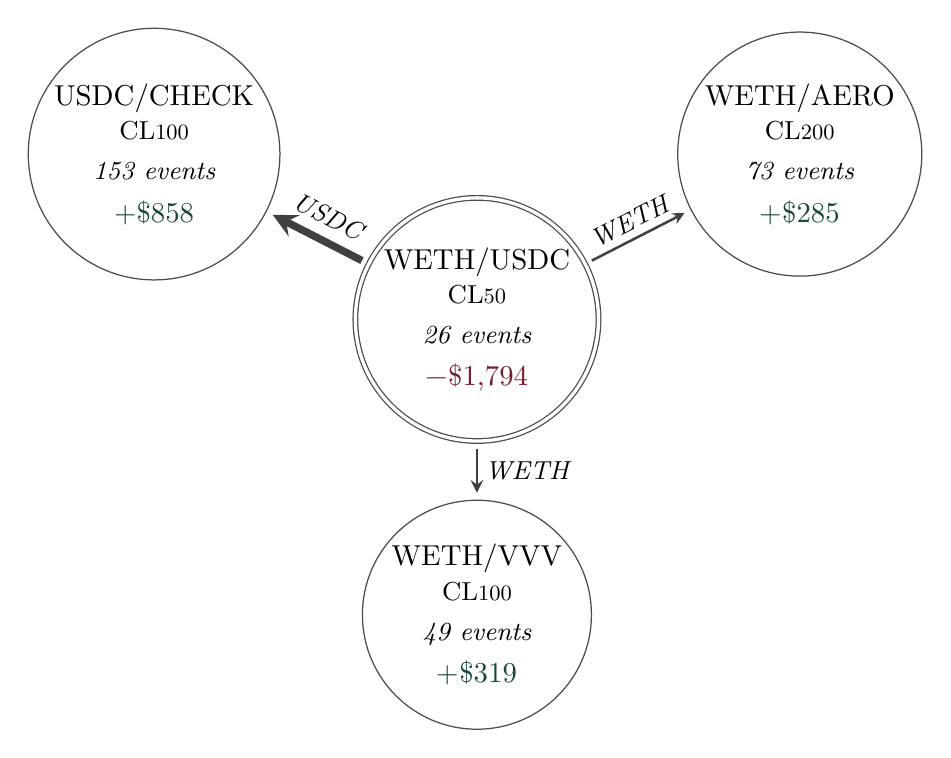
\begin{tikzpicture}[>=to,
  ring/.style = {circle, draw=black!70, line width=0.45pt, minimum size=2.55cm, align=center, inner sep=1pt, font=\small},
  lab/.style  = {font=\footnotesize\itshape, inner sep=2.5pt},
  flow/.style = {-stealth, draw=black!75, shorten >=2.5pt, shorten <=2.5pt}]
\node[ring, minimum size=2.9cm, double, double distance=1.2pt] (h) at (0,0) {\acr{WETH}/\acr{USDC}\\[-1pt]{\footnotesize\acr{CL}\scn{50}}\\[1pt]{\footnotesize\itshape 26 events}\\[2pt]\textcolor{oxblood}{$-$\$1{,}794}};
\node[ring] (s1) at (-4.1,2.1) {\acr{USDC}/\acr{CHECK}\\[-1pt]{\footnotesize\acr{CL}\scn{100}}\\[1pt]{\footnotesize\itshape 153 events}\\[2pt]\textcolor{racing}{$+$\$858}};
\node[ring] (s2) at (4.1,2.1)  {\acr{WETH}/\acr{AERO}\\[-1pt]{\footnotesize\acr{CL}\scn{200}}\\[1pt]{\footnotesize\itshape 73 events}\\[2pt]\textcolor{racing}{$+$\$285}};
\node[ring] (s3) at (0,-3.75)  {\acr{WETH}/\acr{VVV}\\[-1pt]{\footnotesize\acr{CL}\scn{100}}\\[1pt]{\footnotesize\itshape 49 events}\\[2pt]\textcolor{racing}{$+$\$319}};
\draw[flow, line width=2.7pt] (h) -- node[lab, sloped, above=1.5pt] {\acr{USDC}} (s1);
\draw[flow, line width=0.9pt] (h) -- node[lab, sloped, above] {\acr{WETH}} (s2);
\draw[flow, line width=1.0pt] (h) -- node[lab, right] {\acr{WETH}} (s3);
\end{tikzpicture}
\caption{Hub-spoke topology in Group~B (Phase~2). Arrow thickness scales with cumulative absorption, and italic labels indicate the connector token.}
\label{fig:hub-spoke}
\end{figure}

Major hub donations were followed by spoke absorptions within about two hours. This pattern is consistent with \acr{WETH} residuals emitted by the hub being absorbed by \acr{WETH}-paired spokes on subsequent rebalances.

Positions in different pools do not converge to equal value. The hub remains the largest because its pool, \acr{WETH}/\acr{USDC} \acr{CL}\scn{50}, is deeper than the spokes' pools, which gives it a lower $V/L_p$ for the same capital. The heuristic~\eqref{eq:multipool} describes this pattern.

\subsection{Regime analysis}\label{sec:regime}

The 42-hour Phase~1 window can be divided into five market-state sub-periods (Appendix~\ref{app:empirical}, Table~\ref{tab:regime}). On average, volatile positions shed capital during stress and absorbed capital during the subsequent recovery. Flow direction is therefore regime-dependent rather than fixed by position, which is consistent with mismatch widening under stress.

\subsection{Stablecoin \acr{FX} isolation}\label{sec:fx-isolation}

Five stablecoin \acr{FX} pairs deployed over a weekend, when foreign-exchange markets were closed, provide a setting in which the reference rates do not move (Appendix~\ref{app:empirical}, Table~\ref{tab:fx}). The pool prices still moved, and the table gives the engine's volatility for each pool. All 321 fiat rebalances were sent in the contract's automatic swap mode, and 187 of them carry an internal swap in the position's own pool. Of the 49 events in the table's window, 42 carry one (last column of Table~\ref{tab:fx}). The dust flows of the table are therefore net of a swap on most events.

\acr{ZARP} ($L/L_p \approx 0.96$) donated a mean $34\%$ of its value per donation event, \acr{KRWQ} and \acr{CADC} grew, and the portfolio-level dust totals approximately netted out (sum $+\$250$). \acr{ZARP} was almost all of its pool's in-range liquidity, which is outside the first-order domain of Proposition~\ref{prop:leftover}. The pattern agrees with it in direction only, the leftover growing with $L/L_p$.

\subsection{The two-mechanism split}\label{sec:two-mechanism-split}

About half of all rebalances change range. On chain that is 280 of the 642 Phase~2 events ($44\%$) and $20{,}246$ of the $35{,}704$ matched Phase~3 events ($57\%$), and the rest are minted back into the same range. The range changes create nearly all of the geometric residual, between $99.97\%$ and $100\%$ of it in every phase (\S\ref{sec:ledger}).

The dust pool grows on range changes and shrinks on same range rebalances in every phase. On the \acr{PMV}\scn{9} pools with complete coverage the net value absorbed from the dust pool is positive on same range events and negative on range changes, and both intervals exclude zero. The two stages are nevertheless not carried by separate sets of events. A range-change rebalance is missing one token and absorbs it if the dust pool holds it, so range changes account for most of the dust absorbed, between $76\%$ and $93\%$ depending on the phase.

\subsection{Position extinction: the \acr{ZARP} case study}\label{sec:zarp}

The \acr{USDC}/\acr{ZARP} \acr{CL}\scn{10} position of Phase~2 fell from \$942 to \$1.59 over 14 rebalances (Appendix~\ref{app:empirical}, Table~\ref{tab:zarp}). All 14 are range changes. On twelve the position manager's internal swap ran, in the \acr{USDC}/\acr{ZARP} pool itself and for a total of \$931 of \acr{USDC}. On two, events 7 and 14, there was no swap.

The swaps did not recover what a swap at a fixed price would. The position was most of its pool, and its own swap moved the pool price by between 8 and 199 ticks, against ranges mostly 100 ticks wide. On 11 of the 12 the leftover is in the token the swap bought. This is the direction Corollary~\ref{cor:swap-size} gives for a swap larger than $\theta = 1/(1+\lambda)$, although the position was too large relative to its pool for the first-order size to apply. On the events where the position lost value the trajectory is of the kind Proposition~\ref{prop:partial} describes.

On four events (5, 8, 12, and 13) the position grew. The proposition assumes isolated rebalances, so these four lie outside it. They are the position re-absorbing its own stranded swap output from the dust pool, as Corollary~\ref{cor:irreversibility} requires; on one of them it also absorbed \acr{USDC} left by other positions under the same depositor.

In neither of the two zero-swap events had the price left the old range, so they are not instances of Theorem~\ref{thm:extinction}, whose premise is an exit. They test the zero-swap factor $1 - \alpha$ of Theorem~\ref{thm:residual}, which is the factor in the product of Theorem~\ref{thm:extinction}. From the pool state one block before each transaction, Theorem~\ref{thm:residual} gives factors of $0.300$ and $0.006$, and the realised factors equal them to the precision shown.

Two figures set the trajectory beside the bound of Theorem~\ref{thm:extinction}. Neither is a test of it. The bound is the number of rebalances that reach the terminal value of \$1.59 at a constant $\alpha$. At the mean zero-swap residual fraction of the fourteen events, $0.68$, it is 6. At the mean realised $\alpha$ of the ten events on which the position lost value, $0.45$, which includes the effect of the swaps, it is 11. In Table~\ref{tab:zarp} the last column gives the \acr{USDC} amount of each internal swap, from chain and rounded to the dollar, and $\alpha$ is $-D$ over the pre-rebalance value. Total donated was \$1{,}528 and total absorbed \$587, a net of $-\$941$, or $99.8\%$ of initial capital.

\subsection{The exact dust accounting}\label{sec:ledger}

Per rebalance and per token of the pool pair, the contract's accounting gives
\begin{equation}\label{eq:ledger}
D_{\symup{pool}}^{\symup{before}} + \text{withdrawn} + \text{fees} + \text{swap} = \text{mint} + D_{\symup{pool}}^{\symup{after}} ,
\end{equation}
with $D_{\symup{pool}}^{\symup{before}}$ and $D_{\symup{pool}}^{\symup{after}}$ the depositor's dust pool of that token before and after the event. Every term has its own source on chain. The withdrawn and minted amounts come from the position manager's liquidity events, the fees from the pool's \texttt{Collect}, the swap from the pool's \texttt{Swap} or the Odos aggregator's event, and the dust pool from the replayed contract events. The identity is the contract's own arithmetic. Its closure therefore tests whether these records account for the whole token flow, with no unmodelled term, and it is not an empirical law.

It closes to the wei, on both tokens, on about $143{,}000$ \acr{PMV}\scn{9} rebalances, which is every rebalance for which all terms are available. On about $135{,}500$ of them every term is read from an indexed chain event. On the other $7{,}300$ the fee term is implied, and on about 500 of those the swap term is taken from the realised amount recorded in the operator's log, because of a gap in the indexed swap events. The fee term is zero on every one of them, since the positions were staked and a staked Slipstream position collects no fees. On \acr{PMV}\scn{6}--\acr{PMV}\scn{8} it closes on about $24{,}000$ of $26{,}400$ rebalances, and on a further $1{,}000$, all in the \acr{WETH}/\acr{AERO} pool, once the \acr{AERO} emissions that those versions receive in the same transaction are allowed for.

Writing the withdrawn amounts as the part the new range can take with no swap plus a remainder isolates the geometric residual $\Delta R$ of each event exactly. Three results follow.

\textit{Theorem~\ref{thm:residual} on chain.} The residual is negligible on same range rebalances and arises almost entirely at range changes. On the roughly $60{,}000$ same range \acr{PMV}\scn{9} events it has median $1.3 \times 10^{-11}$ of position value and a 99.9th percentile of $9.8 \times 10^{-6}$. Range changes create between $99.97\%$ and $100\%$ of all residual in every phase.

\textit{What the internal swap absorbs.} On range changes, between $98\%$ and $99.7\%$ of the residual is deployed in the mint at the event, depending on the phase, at a swap cost of $0.06\%$ to $0.11\%$ of the residual.

\textit{The leftover, per event.} The companion papers give the leftover of a rebalance executed in a single transaction as the mint minimum~\eqref{eq:mint} applied to the amounts held after the swap, with the required token ratio computed at the current tick.\cite{ryan2026master,ryan2026oqm} The law is evaluated exactly on the events whose pool liquidity along the swap is known from the state before the transaction, first on \acr{PMV}\scn{6}--\acr{PMV}\scn{8}, whose outcomes had not been examined when the test was specified, and then on \acr{PMV}\scn{9} (Table~\ref{tab:leftover-law}).

\begin{table}[!htb]
\centering
\caption{The per-event leftover law against the leftover added to the dust pool.}
\label{tab:leftover-law}
\begin{tabular}{@{}lrr@{}}
\toprule
 & \thd{PMV}\scn{6}\thd{--PMV}\scn{8} & \thd{PMV}\scn{9}  \\
\midrule
Eligible events, rounded                 & $8{,}100$ & $140{,}100$ \\
Leftover token correct                   & $98.4\%$  & $99.2\%$ \\
Predicted over observed amount, median   & $1.0000$  & $1.0000$ \\
Token correct, ``the token the swap bought'' & $84\%$ & $61\%$ \\
\bottomrule
\end{tabular}
\end{table}

\noindent The law names the leftover's token far more reliably than the rule that it is the token the swap bought. On \acr{PMV}\scn{6}--\acr{PMV}\scn{8} the events on which it is right carry $99.4\%$ of the leftover by \acr{USD} value, and both quartiles of the amount ratio are $1.0000$. The first-order form of Proposition~\ref{prop:leftover} matches the leftover in aggregate amount and gives the wrong token on a third of \acr{PMV}\scn{9} swaps. The tick-rounding term it omits changes the leftover's token on about a third of swaps, and with it the positions that can absorb the leftover.

The test set in advance for the law on \acr{PMV}\scn{6}--\acr{PMV}\scn{8} contained one criterion that cannot be met. It required the rank correlation of predicted with observed leftover to be $0.05$ above that of a baseline, which stood at $0.957$, so the test did not pass as specified. The law's correlation was $0.998$, and every other criterion was met.

\subsection{Transfer and return attribution}\label{sec:transfer}

Proposition~\ref{prop:neutral} defines the transfer at a rebalance as the part of the mint above the position's own equity. Carrying an entitlement for every position through the replayed \acr{PMV}\scn{9} dust pool, as described after Proposition~\ref{prop:neutral}, gives the transfer between every pair of positions in a portfolio over the life of the deployment. Table~\ref{tab:transfer} sets that definition beside two others, each summed over absorbers from 21~March to 14~October 2026. The second follows each token from the rebalance that left it to the rebalance that absorbed it. The third also counts as transfer the \acr{AERO} emissions that were paid into the dust pool and absorbed by a position other than the one that earned them.

The third definition has its own base for comparison. Under one arrangement emissions were paid out at each rebalance, and under a later one they were sold and the proceeds paid into the dust pool. Ten positions passed from the first arrangement to the second during the period. The third definition counts each of the ten as two positions, one under each arrangement. On positions divided in that way the first definition gives \$122{,}940.

\begin{table}[!htb]
\centering
\caption{Net transfer between positions on \acr{PMV}\scn{9}.}
\label{tab:transfer}
\begin{tabular}{@{}lr@{}}
\toprule
\thd{Definition} & \thd{Net transfer (USD)}  \\
\midrule
Above own equity   & 121{,}530 \\
Token tracing      & 132{,}126 \\
Above own equity, with emissions & 112{,}766 \\
\bottomrule
\end{tabular}
\end{table}

\noindent Gross transfers were much larger than the net. Of the \$12.9 million that positions drew from the dust pool, \$4.3 million came from the entitlements of other positions. Most of it is offset by what the same positions gave up to others, and the net transfer is about $0.9\%$ of the value drawn. Fifteen per cent of rebalances minted above own equity. The transfer is zero-sum within each dust pool at every rebalance, under every definition, since what one position receives is debited from the others. The same positions are donors and absorbers under the first two definitions in 100 of 108 cases.

Because the transfer is zero-sum, it does not change what the positions sharing a dust pool keep between them. It changes which position appears to have kept it. Define a position's \emph{own return} as its emissions less its loss-versus-rebalancing, estimated from the pool price 300 seconds after each swap, less its swap cost, and its \emph{realised return} as its own return plus its transfer. Loss-versus-rebalancing is the measure of Milionis et al.\cite{milionis2022b} Fritsch and Canidio\cite{fritsch2024} estimate it for passive liquidity against an exchange reference price, and the estimate here uses the pool's own later price.

Across the 107 positions of at least seven days, own return and realised return have a Spearman correlation of $0.02$. The transfer changes the sign of the estimated return of 52 of the 107 positions and moves 73 by ten or more places in rank. On this dataset a position's realised return is nearly uncorrelated with its own return.

Three checks vary the aggregation, the horizon, and the treatment of emissions. Aggregated to the 70 pools, the correlation is $0.12$ and the estimated return of 30 pools changes sign. With the loss estimated at horizons of 60, 300, and $3{,}600$ seconds, between 46 and 52 positions change sign. Across the 86 position-periods in which emissions were paid out at each rebalance the correlation is $-0.06$, and across the 30 in which they were paid into the dust pool it is $+0.25$, with intervals that overlap. In each check the association between own return and realised return stays weak.

The direction of the transfer follows from the accounting. A position's equity is net of its own swap slippage (Proposition~\ref{prop:neutral}). Under~\eqref{eq:mint}, a position with no entitlement that mints back the value it withdrew has therefore minted above its equity by exactly its slippage $S_j$, and that amount comes from the entitlements of the other positions.

The data agree in sign and in rank. The rank correlation of transfer with swap cost is $+0.31$ within portfolios and $+0.26$ across the 107 positions. The 50 net absorbers have a median swap cost of $320\%$ of position value a year, against $131\%$ for the 57 net donors, each position's cost being divided by its value integrated over the time it was open. Transfer and own return are rank-correlated at $-0.34$ within portfolios, so the transfer runs towards the positions with the lower own return. With emissions less loss alone the correlation across positions is $-0.07$. The share of swap cost passed on in this way is not measured.

\subsection{Which positions donate}\label{sec:prediction}

If the leftover is known per event, the transfer follows from which position absorbs which leftover. A position's net transfer can then be predicted from the state before each rebalance and the recorded order of rebalances, with no observed leftover as an input. Two prediction models were evaluated. The specification and thresholds of each were fixed before the outcomes of its first test were examined, in the manner of a preregistered analysis.\cite{nosek2018}

The first model used the first-order law of Proposition~\ref{prop:leftover} with the rule that the leftover is the token bought. Tested on \acr{PMV}\scn{9}, it failed. The within-portfolio rank correlation of predicted with observed transfer was $+0.08$, with a permutation $p$-value of $0.28$, against a threshold of $0.28$ for the correlation set in advance. Two single variables each did better, the position's liquidity relative to its pool's, with sign reversed, at $+0.28$, and its range width at $+0.27$. Across the 21 portfolios the model's predicted and observed net transfer had a rank correlation of $+0.96$, and the predicted transfer was about ten times the observed. It placed the leftover in the wrong token on a third of swaps, which assigns the leftover to the wrong absorbing position.

The second model used the exact per-event law of \S\ref{sec:ledger}. It was tested first on \acr{PMV}\scn{6}--\acr{PMV}\scn{8}, which neither the theory nor the first model had used, and that test is out of sample. The \acr{PMV}\scn{9} test uses the same code unchanged and is not out of sample, since \acr{PMV}\scn{9} outcomes had already been examined.

The thresholds were set in advance to apply to a restricted sample, the portfolios in which the events the law treats exactly carry at least three quarters of the predicted leftover. Those events are the eligible events of Table~\ref{tab:leftover-law} and the rebalances on which the contract makes no swap. The restriction selects 135 of 288 positions on \acr{PMV}\scn{6}--\acr{PMV}\scn{8} and 60 of 105 on \acr{PMV}\scn{9}, and Table~\ref{tab:prediction} reports those samples. Correlations are taken within portfolio, with one-sided permutation $p$-values, and the two baselines are the single variables above. The last three rows are medians, over portfolios for the ratio of observed to predicted transfer and over positions for the share of a position's intake that is its own leftover.

\begin{table}[!htb]
\centering
\caption{Predicted against observed net transfer per position.}
\label{tab:prediction}
\begin{tabular}{@{}llrr@{}}
\toprule
 & \thd{Criterion} & \thd{PMV}\scn{6}\thd{--PMV}\scn{8} & \thd{PMV}\scn{9}  \\
\midrule
Positions tested                 &                & 135      & 60 \\
Rank correlation                 & at least $0.28$ & $+0.326$ & $+0.484$ \\
Permutation $p$                  & below $0.05$   & $0.0002$ & $0.0004$ \\
Baseline, liquidity              &                & $+0.247$ & $+0.258$ \\
Baseline, range width            &                & $+0.095$ & $+0.230$ \\
Sign agreement                   & above $0.5$    & $0.692$  & $0.650$ \\
Observed over predicted          & $0.40$ to $2.5$ & $0.56$  & $0.37$ \\
Own-leftover share, predicted    &                & $0.393$  & $0.592$ \\
Own-leftover share, observed     & within $0.10$  & $0.547$  & $0.571$ \\
\bottomrule
\end{tabular}
\end{table}

\noindent In these samples the model separates the positions that pay from those that receive, and it ranks them better than either baseline on both datasets. On all positions the rank correlation is $+0.235$ on \acr{PMV}\scn{6}--\acr{PMV}\scn{8} and $+0.384$ on \acr{PMV}\scn{9}, above both baselines on each dataset and, on \acr{PMV}\scn{6}--\acr{PMV}\scn{8}, below the threshold of $0.28$.

The model does not size the transfer consistently. Its prediction is about $1.8$ times the observed transfer on \acr{PMV}\scn{6}--\acr{PMV}\scn{8}, inside the band set in advance, and about $2.7$ times on \acr{PMV}\scn{9}, outside it. The predicted share of a position's intake that is its own leftover is the reverse case, further than $0.10$ from the observed share on \acr{PMV}\scn{6}--\acr{PMV}\scn{8} and within it on \acr{PMV}\scn{9}. The model meets its ranking and sign criteria on both datasets, and each of its two size criteria on one.

\subsection{Convergence and mechanism tests}\label{sec:simulator}

\acr{PMV}\scn{9} contains three pairs of positions in one pool and one portfolio that were open together and rebalanced at similar rates, the premise of Theorem~\ref{thm:convergence}. Valued from chain amounts alone, the value gap of each pair contracts (Table~\ref{tab:pairs}). In each pair the fitted rate per own rebalance exceeds the donation rate of Corollary~\ref{cor:convergence-rate} estimated on the same events, and the bootstrap intervals of the two rates do not overlap. Nothing is transferred on the 629 same range zero-swap rebalances in these pairs. The contraction therefore occurs inside rebalances that swap or change range, and it is not the proportional donation on same range events that the model assumes.

The pairs do not settle at equal value, as Corollary~\ref{cor:dispersion} allows. The observed gap of Table~\ref{tab:pairs} is the root-mean-square relative gap over the second half of each sample. The stationary level is that of the bound of Corollary~\ref{cor:dispersion}, estimated from the same events with the noise of the per-event donation included. The observed gaps of the second and third pairs lie inside the interval of the estimate. That of the first, $0.170$, is above the upper end of its interval, $0.166$.

\begin{table}[!htb]
\centering
\caption{Value gap of three same-pool pairs on \acr{PMV}\scn{9}, with bootstrap intervals. Event counts are rounded.}
\label{tab:pairs}
\begin{tabular}{@{}lrrrrr@{}}
\toprule
\thd{Pair} & \thd{Events} & \thd{Fitted rate} & \thd{Donation rate} & \thd{Observed gap} & \thd{Stationary level}  \\
\midrule
1 & 48{,}000 & $0.112$ & $0.068$ & $0.170$ & $0.157$ \\
  &          & ($0.101$, $0.126$) & ($0.061$, $0.073$) & & ($0.148$, $0.166$) \\
2 & 1{,}100  & $0.233$ & $0.032$ & $0.120$ & $0.139$ \\
  &          & ($0.134$, $0.343$) & ($0.022$, $0.045$) & & ($0.098$, $0.182$) \\
3 & 530      & $0.357$ & $0.031$ & $0.384$ & $0.312$ \\
  &          & ($0.248$, $0.485$) & ($-0.012$, $0.163$) & & ($0.226$, $0.391$) \\
\bottomrule
\end{tabular}
\end{table}

\noindent The simulator of \S\ref{sec:foundry} removes the components of Table~\ref{tab:siphon-components} one at a time. Each run holds four positions of sizes $1{:}2{:}3{:}4$ in one pool for about 350 rebalances per position. The grid crosses seven swap rules with three range widths, three volatilities, and five values of the positions' combined liquidity relative to the rest of the pool's, from $10^{-3}$ to $10$. The swap rules are no swap, the contract's internal swap scaled to $0.25$, $0.5$, $0.75$, $0.9$, and $1$ of its amount, and a swap that matches the new range exactly at no cost. That gives 315 combinations, 45 for each swap rule. Each is run 16 times with the dust pool shared and 16 times with it isolated per position. A combination is counted as converging when the median position keeps at least half its value and the dispersion of the positions' values at least halves, and as holding when the dispersion does not halve.

The simulated positions show the same excess of the fitted rate over the donation rate as the three pairs. With the contract's internal swap and groups of 2 to 16 positions on one range, the fitted rate is between $1.2$ and $2.5$ times the donation rate, and its bootstrap interval excludes the donation rate at every group size.

Convergence requires a leftover. Under the ownerless rule and the contract's internal swap at its full amount, positions converge in 37 of the 45 combinations, and in every combination where the positions together are at most a tenth of the pool the outcome is convergence or holding. A swap that matches the new range exactly leaves nothing over, and the positions then hold their values and never converge.

Redeployment requires a swap. With none, the deployed positions go extinct in every combination, their value stranded in the dust pool. In a single pool every position is missing the same token at once, so the surplus token cannot be redeployed without a swap. Theorem~\ref{thm:extinction} does not cover this case, since the balance is shared. Its own case is the isolated dust pool. On all $2{,}880$ simulated positions with an isolated dust pool and no swap, the final value is the initial value times the product $\prod_k (1 - \alpha_k)$ of Theorem~\ref{thm:extinction} exactly, and its bound holds on every one. With the dust pool isolated, every swap of at most $0.9$ of the contract's amount also leads to extinction.

The transfer is the third component. With the neutral rule of Proposition~\ref{prop:neutral} in place of~\eqref{eq:mint}, the net transfer is below $10^{-9}$ of value on every one of the $5{,}040$ runs with a shared dust pool. Under the ownerless rule 95 of the 315 combinations converge, and under the neutral rule none of them does. In the simulation, convergence under a shared balance is produced by the transfer alone.

A replay of about $135{,}500$ \acr{PMV}\scn{9} rebalances shows a large reduction in the value minted above own equity, and it does not meet the reproduction criterion set for it in advance. With the neutral rule off, the replay should return the realised mints. It does so exactly on $35.5\%$ of events, against the $90\%$ set in advance, with a median relative error of $0.12\%$. A difference of one unit in a portfolio's balance carries into every later event. With the rule on, the gross value minted above own equity falls from about \$1.6 million to under \$2{,}000. Both figures come from the replay and carry its error.

In the form used above, a cap on the contract's own mint, the neutral rule can raise the value swapped, by $6.4\%$ on the replay. A second form lowers it. Applied so that a position takes only its missing token from the dust pool, up to its missing amount, and swaps only its own withdrawn amounts, it lowers the value swapped by $1\%$ to $35\%$ across the grid. On simulated portfolios run under the contract's rules, almost none of the saving of Proposition~\ref{prop:netting} is realised. The shared balance lowers the value swapped by $0.35\%$, against about a tenth available, and swap cost is $22\%$ higher than with isolated balances, because the contract's internal swap is sized on the whole dust pool at every event.

\subsection{Shared tokens on the on-chain dataset}\label{sec:connector-test}

The test of the Connector conjecture of \S\ref{sec:connector} was specified in full before it was run. A pool-group combination is a pool within a depositor group, and its observed driver is the token whose \acr{USD} flow to the dust pool correlates more strongly with the group's total flow, the form in which Table~\ref{tab:cross-group} reports it. Of 101 combinations with at least 30 events and a unique more-connected token, the conjecture names the driver in 54 (binomial $p = 0.55$), which is not distinguishable from chance. Three variants of the test give the same answer, 59 under a rank correlation, 55 by gross \acr{USD} flow, and 53 of 90 with connectivity counted at the time of each event. The \acr{WETH}/\acr{USDC} pool appears in 19 combinations across 13 portfolios, and the observed driver is \acr{WETH} in 7 of the 9 where the conjecture predicts \acr{WETH} and in 7 of the 9 where it predicts \acr{USDC}. In the simulator, across $38{,}045$ combinations in $12{,}000$ random portfolio graphs, the conjecture names the driver in $34.5\%$, and its success falls as the gap in connectivity widens. On the group mapping of the data deposit, four of the nine rows of Table~\ref{tab:cross-group} go against the conjecture. The test above scores connectivity alone. The condition of Corollary~\ref{cor:shared} concerns returns and has not been scored on the dataset.

\subsection{Dust flow and Theorems~\ref{thm:directional} and~\ref{thm:exit}}\label{sec:directional-empirical}

Theorems~\ref{thm:directional} and~\ref{thm:exit} concern the value of a displaced or exited position, and they are verified in exact arithmetic and on a live pool in \S\ref{sec:foundry}. Dust flow at a rebalance with an internal swap is a different quantity, governed by the leftover of \S\ref{sec:leftover}, and for a range centred on the price Proposition~\ref{prop:leftover} has no direction. The companion paper on the position manager's swap sizing shows that the side of the leftover is set by a race between the rounding of the target ratio to the floor tick and the swap's own displacement of the price.\cite{ryan2026oqm} A second effect is the placement of the new range, whose bounds lie on whole tick spacings and whose centre is therefore offset from the price. In the simulator the sign of rising-minus-falling dust follows that offset and reverses when a pool is moved from negative to positive ticks. Under the contract's swap rule, none of the $6.8$ million displaced or exited rebalances in the simulation was made without a swap, so the zero-swap setting of the two theorems does not arise there. Comparisons of dust on rising and falling rebalances, or on above-range and below-range exits, therefore do not test the theorems in either direction. The per-portfolio comparisons of the May 2026 version are given on chain-derived displacement and exit sides in Appendix~\ref{app:changes}.

\section{Computational verification}\label{sec:foundry}

Theorems~\ref{thm:residual} and~\ref{thm:extinction}--\ref{thm:exit} are computationally verified through a 16-test Foundry suite, six of whose tests run against unmodified Aerodrome Slipstream contracts, a V3 fork, on Base mainnet. Theorem~\ref{thm:convergence}, a statement in expectation over many rebalances, is outside the suite and is covered by the Lean formalisation. The canonical example, Test~1, mints a 1 \acr{WETH} $+$ 2{,}500 \acr{USDC} position across $\pm 500$ ticks around tick 73{,}135, displaces the price by $+200$ ticks, and rebalances into a $\pm 1{,}000$-tick range, returning 2{,}061 \acr{USDC} to the depositor balance as the geometric residual. The control test (same setup, re-mint into the identical range) returns 29 base units of \acr{USDC} ($<\!10^{-4}$ \acr{USD}), the analytical zero up to integer-arithmetic floor.

The suite covers Theorems~\ref{thm:residual} and~\ref{thm:extinction} with mock-pool tests, and Theorem~\ref{thm:residual} and the architectural precondition with four live fork tests against the Aerodrome Slipstream \texttt{NonfungiblePositionManager}. It covers Theorems~\ref{thm:monotonicity}--\ref{thm:exit} with mock-pool tests using exact V3 \texttt{TickMath} constants, together with two further live fork tests on the Slipstream \acr{WETH}/\acr{USDC} pool for the directional and exit asymmetries, bringing the fork-test total to six.

All six fork tests are pinned to Base block \texttt{43{,}175{,}000} (2026-03-10 10:42 \acr{UTC}), inside the paper's Phase~2 data window, so both the qualitative claims and the captured numerical residuals are reproducible against an archive \acr{RPC}. Test descriptions and assertion details are in Appendix~\ref{app:foundry-detailed}, and reproduction commands in Appendix~\ref{app:foundry}.

The leftover and the transfer are checked with an exact simulator of the rebalance, an integer port of the pool's tick, swap, mint, and burn arithmetic together with the position manager's sizing and swap rules. It is replayed on about $133{,}300$ \acr{PMV}\scn{9} rebalances whose pre-transaction pool price is verified against chain.

Three comparisons are made. Stage by stage, with each stage given the chain's state at its start, the simulator reproduces the contract's swap decision, direction, and amount on every event, and the mint's liquidity and leftover on every event. As a reconstruction conditioned on two observed inputs, the pool's liquidity from the transaction's swap event and the fee identified per swap, simulated dust per event equals the on-chain value to the wei on $94.7\%$ of events, and every remaining miss is a swap whose fee cannot be identified in one step. In a sample of such swaps most crossed an initialised tick or had their fee changed inside the block, and about a third were not explained. As a prediction from the pre-transaction state alone, with the pool's liquidity taken from the preceding swap, the leftover is exact on $66.3\%$ of events.

A parallel implementation agrees with the reference bit for bit on 256 random portfolios. The simulator is used in \S\ref{sec:simulator} to switch the three components of Table~\ref{tab:siphon-components} off one at a time.

The simulator also measures the accuracy of two propositions. The first-order leftover of Proposition~\ref{prop:leftover} agrees with the simulated leftover where the position's liquidity is between $10^{-3}$ and $10^{-1}$ of the pool's, with a median ratio of observed to predicted leftover of $0.96$ to $1.01$. Below that range rounding and the fee are as large as the price impact, and above it the price impact is no longer first order. Sizing the swap at $\theta = 1/(1+\lambda)$ reduces the median leftover by a factor of 11 to 59 inside that range, and reduces the net transfer by a factor of 2.4 to 6 where the positions are at least as large as the rest of the pool. Proposition~\ref{prop:excursion} holds to a median relative error of $3 \times 10^{-17}$ on 680 in-range excursions in integer arithmetic.

\section{Discussion}\label{sec:discussion}

The results separate three quantities. The residual is created by a rebalance that changes the required token ratio. The leftover is what the internal swap fails to redeploy. The transfer is what a shared balance with no record of ownership lets another position take. The first follows from the amount equations and is the same for every position manager. The other two depend on the position manager, through its swap and its accounting. That separation decides which findings extend to other implementations and which are specific to the deployment studied, and the rest of this section follows it.

\subsection{The architectural precondition}\label{sec:precondition}

The geometric residual arises on any \acr{CL} rebalance that changes the required token ratio at the current price, and in that sense it has existed since Uniswap V3 launched in May 2021. In vault-per-pool architectures, it remains trapped within the position that produced it and usually appears only as a small capital efficiency loss, hard to distinguish from slippage in standard PnL tracking. Depositor-level shared balances change that. They let a residual from one pool be absorbed by a position in another, where it becomes visible as a flow between positions.

Theorem~\ref{thm:residual} applies to all Uniswap V3-style concentrated liquidity implementations. Its argument uses only that a deposit must be made in proportions fixed by the price, so the residual belongs to any fixed-proportion deposit. Cross-position flow further requires shared token balances across positions in different pools, with no entitlement recorded per position (Proposition~\ref{prop:neutral}). Depositor-level multi-pool accounting is still uncommon in production \acr{CL} management, but it is not unique to the \acr{PMV}\scn{6}--\acr{PMV}\scn{9} family studied here; any protocol that adopts it becomes exposed to the same mechanism.

The fork test in \S\ref{sec:foundry-fork} checks this precondition directly. On a stock \acr{NFPM}, which does not maintain shared depositor balances, no cross-position absorption occurs. A concurrent \acr{SSRN} preprint\cite{secondoperator2026} formalises a graph-theoretic condition for cross-pool circulation (token degree $\geq 2$ in the portfolio graph) on a port of the Position Manager to Uniswap V3, and derives a directional-convexity scaling for symmetric sqrt-price displacements. Its circulation condition is the necessity half of Proposition~\ref{prop:netting}. That work does not address quantitative magnitudes.

\subsection{What the transfer explains}\label{sec:transfer-discussion}

A residual arises when a range change alters the required token ratio, and the internal swap absorbs almost all of it. The transfer is built from the remainder. The size of that remainder depends on the position manager, through the swap sizing of Proposition~\ref{prop:leftover} and the tick-rounding term of the companion papers, and a position manager that sized its internal swap for its own price impact would leave less.

At each rebalance the transfer redistributes value among the positions sharing a dust pool and leaves their combined value unchanged. It is therefore not what a portfolio loses. That is the cost of rebalancing along the price path, whose accounting belongs to the companion paper on rebalancing cost.\cite{ryan2026localtime} The shared balance can still change later swap costs and the capital left undeployed (\S\ref{sec:simulator}), and those are effects of the design and not of the transfer.

What the transfer explains is the dispersion of realised returns among the positions of one portfolio. A position's apparent performance can include value supplied by other positions, and on this dataset a position's realised return is nearly uncorrelated with its own return (\S\ref{sec:transfer}). Two consequences follow. Under the ownerless rule a position can recover its swap slippage from the other positions in its portfolio. The share of swap cost passed on in this way is not measured here, but the net absorbers tend to be the positions with the higher swap cost, so a rule that allocates capital on realised returns can favour positions that are expensive to rebalance. Cross-subsidy of weaker units by stronger ones is a known failure of internal capital markets.\cite{scharfstein2000} Where the positions sharing a dust pool have different owners, the transfer is also a transfer of wealth between them. The neutral rule of Proposition~\ref{prop:neutral} prevents both.

\subsection{Boundary cases}\label{sec:boundary}

Three observations from Phase~1 mark the edges of the mechanism. Two \acr{EURC}/\acr{USDC} \acr{CL}\scn{1} positions in the same pool passed dust back and forth, consecutive events reversing sign $62\%$ of the time, which produced dissipation and no reallocation between pools. The cbETH/cbBTC position donated \$2{,}413 that no other position could use, because none held cbETH, and it accumulated as contract dust. A token must be held by at least two positions before it can carry flow between them (Proposition~\ref{prop:netting}). Per-event flows are also heavy-tailed, two of \acr{FLOCK}'s 23 rebalances accounting for $96\%$ of its lifetime donation.

\subsection{Direction, magnitude, and unit of account}\label{sec:direction-discussion}

The siphon moves tokens between positions according to geometric ratios, and it is blind to direction. Theorems~\ref{thm:directional} and~\ref{thm:exit} concern a different quantity, the value of a displaced or exited position in a stated unit of account, and their inequalities reverse when the unit changes. The dust left by a rebalance with an internal swap is a separate quantity again. Its token and amount are set by the sizing of the swap, by tick rounding in the target ratio, and by the placement of the new range (\S\ref{sec:directional-empirical}).

Dust performance reported in \acr{USD} therefore combines the flow set by geometry with the price exposure of the tokens moved. \acr{USD} value is economically meaningful, but the direction it shows depends on the unit. Separating the two requires num\'eraire-invariant accounting or explicit segmentation by pool address ordering. Neither is standard in current \acr{LP} performance reporting.

Redeployment carries the same asymmetry. Either terminal exit can only be reopened in range by swapping into the missing token. Above-exits hold the full stablecoin balance, while below-exits hold only the depreciated volatile token. By Corollary~\ref{cor:exit-ratio}, redeployable capital at a below-exit displacement $d$ is a fraction $P'/\sqrt{P_a P_b}$ of the above-exit case and vanishes as the price moves further past the lower boundary. Across consecutive below-exits without a recovery move, the gap compounds. The compounding gap is the operational signature of Theorem~\ref{thm:exit} in a depreciating market.

\subsection{Implications}\label{sec:implications}

\textit{Ownership and attribution.} A shared balance that records no owner hands every leftover, at no charge, to the next position that can use it. Proposition~\ref{prop:neutral} supplies the missing record, the entitlement, valued in one num\'eraire at the prices of the transaction, and Corollary~\ref{cor:unique} shows that the rule is fixed at every rebalance, with only the division of the balance's revaluation between rebalances left as a choice. A shared balance can then net the needs of its positions without one position deploying value owed to another. For a single owner this is a matter of attribution, and \S\ref{sec:transfer} shows how far attribution can be wrong without it. Where the positions under one balance have different owners, or are charged fees or judged separately, the same quantity is a transfer of wealth, and the entitlement is the accounting that a vault with several depositors, a fund with several strategies, or a protocol holding a common balance would need. It requires a price for each token that resists manipulation, which is the difficult part on chain.

\textit{Swap sizing and netting.} Two quantities in this paper are choices of the position manager and not properties of the geometry. Corollary~\ref{cor:swap-size} gives the swap size at which the leftover vanishes to first order, apart from the tick-rounding term, and Proposition~\ref{prop:netting} the least value that a group of positions needs to swap. The deployed contract uses neither, and \S\S\ref{sec:simulator} and~\ref{sec:foundry} measure what each is worth in simulation. A position manager built on them could swap less and leave less. How much netting is available depends on the portfolio. By Corollary~\ref{cor:shared}, for positions rebalanced together, a token nets when its return lies between those of its partners, which is the place of a quote token whenever the assets held against it move apart. Portfolios of stablecoin foreign-exchange pairs, of tokenised equities, or of any set of assets quoted against one token have that graph, and whether their returns straddle the quote token often enough is an empirical matter. The condition is of the kind that governs any netting arrangement, in which the benefit depends on which exposures are pooled.\cite{duffie2011}

\textit{Retained leftover.} Proposition~\ref{prop:excursion} concerns a position that starts fully deployed and keeps its own leftover. While the price stays inside its range, such a position can follow the price with no swap, at a cost held as undeployed capital, not lost. What a move sets aside is first order in the move and returns if the price reverses, and what does not return is second order. Within those conditions, rebalancing without trading is available where a swap is costly, restricted, or unavailable, as in thin pools and for assets whose market is closed for part of the day. The proposition does not cover a price that leaves the range.

\subsection{Limitations}\label{sec:limitations}

The measurements at scale come from one operator's contract family on Aerodrome (Base), across four contract versions, \acr{PMV}\scn{6} to \acr{PMV}\scn{9}. Theorem~\ref{thm:residual} guarantees that the residual exists on all V3-style implementations, and the propositions are properties of the amount equations and of the accounting. The size of the leftover and of the transfer, and the case-study magnitudes, are specific to this position manager's swap sizing and may differ under other protocols, fee structures, rebalancing engines, or pair compositions. The architecture is also in production outside this programme. Crossbow Finance, a concentrated liquidity vault protocol on a second chain, keeps each depositor's dust in a balance keyed by token and shared across that depositor's pools, and its public documentation describes the recycling of residuals between pools.\cite{crossbow2026} On its on-chain record the ledger identity of \S\ref{sec:ledger} closes exactly on every transaction examined. Its venues, pairs, and rebalancing policy differ from those studied here, and the magnitudes of \S\ref{sec:results} are not claimed for it. The ledger identity is computed in tokens from chain events alone, which is what allows the accounting of a deployment, though not the attribution of its profit, to be checked without its operator's records.

The controlled phases cover between two and twelve days and the on-chain dataset seven months, which does not span a full market cycle. Every \acr{PMV}\scn{9} position was staked and collected no trading fees, so the fee term of the ledger is not exercised. The ledger identity of \S\ref{sec:ledger} is established on about $143{,}000$ of approximately $280{,}000$ \acr{PMV}\scn{9} rebalances, those for which every term is available. The adaptive rebalancing engine also creates a circular dependence between volatility, range width, and dust flow.

Several analytical results hold under assumptions that the deployed contract does not meet. Theorem~\ref{thm:extinction} is proved for zero-swap rebalances, and Proposition~\ref{prop:partial} extends it to the intermediate case $0 < S_{\symup{eff}} < 1$. On chain, its zero-swap factor is observed on two zero-swap events (\S\ref{sec:zarp}), neither of them an exit, and the theorem itself is checked in simulation. Proposition~\ref{prop:leftover} is first order and omits the tick-rounding term, for which the companion papers give the exact law. Theorem~\ref{thm:convergence} and Corollary~\ref{cor:convergence-rate} are statements of a model in which the donation rate is constant per unit of value, and the contraction observed on chain is faster than that model's and occurs at range changes (\S\ref{sec:simulator}). Within the model the fixed point, equal value, does not depend on the rate. A single pair is not expected to reach it, and Corollary~\ref{cor:dispersion} bounds how far from it a pair remains. Proposition~\ref{prop:excursion} is verified in exact arithmetic and in simulation and has no test on chain. No zero-swap excursion inside the range from a fully deployed start has been identified in the dataset. The per-event law is evaluated for a position manager that withdraws, swaps, and mints in one transaction. The test specified in advance also covered a second form of the law, for a position manager that swaps and mints in separate transactions, on the deployment noted above. That form did not meet its thresholds for the token of the leftover, for its size, or for its dependence on the price move between the swap and the mint, and the transfer prediction of \S\ref{sec:prediction} had too few positions there for a verdict. In a check not specified in advance, the mint minimum applied to the amounts actually held after the swap reproduces the leftover there to within $1\%$ on every rebalance examined, so the second form fails on the amounts held after the swap, at a tolerance finer than the one at which its sizing rule was met, and not on the mint. The rebalancing policies of other managers are recovered from public data in a companion paper.\cite{ryan2026of}

The prediction, the counterfactual, and the return comparison each establish less than their headline figures. The prediction of \S\ref{sec:prediction} meets its ranking and sign criteria on the restricted samples its thresholds were set for. On all positions its rank correlation on \acr{PMV}\scn{6}--\acr{PMV}\scn{8} is below the threshold, and it does not size the transfer consistently. The counterfactual with per-position accounting is available in simulation and as a replay of the on-chain dataset (\S\ref{sec:simulator}), not as a live run. The replay returns the realised mints exactly on $35.5\%$ of events, against $90\%$ set in advance, so its estimate of the value minted above own equity carries an error that is not bounded here. The simulator is exact in the contract and pool arithmetic and stylised in its market, with independent price paths, pools held at the fair price by arbitrage, and constant outside liquidity, and its regime counts and its score of the Connector conjecture are properties of that model. The comparison of own return with realised return in \S\ref{sec:transfer} uses an estimate of loss-versus-rebalancing that depends on its horizon, and the count of sign changes is reported at three horizons for that reason.

Theorems~\ref{thm:directional} and~\ref{thm:exit} are proved in token1 units. Measured in token0 units, the inequalities reverse, so the asymmetry is a consequence of the chosen unit of account. The \acr{USD} interpretation holds when token1 is \acr{USDC}, \acr{USDT}, or \acr{DAI}, or when token1's \acr{USD} price is approximately stable over the rebalance interval. Neither theorem is tested by the on-chain dataset. Both concern the value of a displaced or exited position at a zero-swap rebalance, and dust flow at a rebalance with a swap is a different quantity (\S\ref{sec:directional-empirical}). Their evidence is the proofs and the computational verification of \S\ref{sec:foundry}.

\subsection{Future work}\label{sec:future}

The first test is a live one. The transfer is zero-sum within a dust pool at each rebalance (\S\ref{sec:transfer}), so the net effect of a shared balance lies in the two quantities it does change, the value swapped and the capital left undeployed. In simulation the contract's rules reduce the value swapped by $0.35\%$, against about a tenth available under Proposition~\ref{prop:netting} (\S\ref{sec:simulator}). A live comparison of a shared balance under the neutral rule of Proposition~\ref{prop:neutral} against vault-per-pool accounting, over a full market cycle, would show whether the saving from netting is worth its cost in swaps and undeployed capital.

A second open question is strategic manipulation. An attacker able to coordinate rebalance timing across multiple positions may be able to extract value from the siphon, but the feasibility, cost, and practical constraints of such an attack are not treated here. Under the ownerless rule the next position that can use a leftover takes it, so with more than one owner the timing of rebalances is strategic, and Proposition~\ref{prop:neutral} gives the accounting that removes the incentive.

On the modelling side, Propositions~\ref{prop:partial} and~\ref{prop:leftover} supply, to first order, the model of swap absorption that interpolates between Theorems~\ref{thm:convergence} and~\ref{thm:extinction}. The per-position prediction should be extended from ranking to size. Corollary~\ref{cor:shared} states when a shared token nets, for positions recentred together, and that condition has not been tested on the dataset. The test needs the value netted per token and per event, which the per-token ledger of \S\ref{sec:ledger} supplies. A first test of the law on a design that separates the swap from the mint did not pass (\S\ref{sec:limitations}), and a law for the leftover in such designs remains open. Proposition~\ref{prop:excursion} has yet to be observed on chain, which needs a position that makes a zero-swap excursion inside its range from a fully deployed start.

Outside concentrated liquidity, the mechanism needs only a deposit that must be made in fixed proportions, proportions that move with a price, and a leftover pooled with no record of its owner. Subscription in kind to a basket fund and accounts that net the balances of several owners have all three. Whether the residual and the transfer are material there is open.

\section{Conclusion}\label{sec:conclusion}

The Geometric Siphon arises when the residual tokens of rebalances that change the required token ratio enter a shared balance and are redeployed by other positions. The V3 amount equations determine the residual, and the internal swap determines what is left undeployed. Six theorems characterise the residual, its growth with displacement, convergence in expectation under a shared balance, extinction without a swap, and the directional and exit asymmetries in a stated unit of account. Six propositions follow the residual through the swap and the mint, and separate these properties of the geometry from the position manager's allocation of the leftover. A Lean formalisation covers the theorem layer in real arithmetic, and a Foundry suite checks Theorems~\ref{thm:residual} and~\ref{thm:extinction}--\ref{thm:exit} in pool arithmetic, in part against unmodified Slipstream contracts.

The controlled experiments and the seven-month on-chain record establish the mechanism in the contract family studied. The reconstructed residual is negligible on unchanged ranges, and on \acr{PMV}\scn{9} the token accounting closes exactly on every rebalance for which all terms are available. Under the equity definition about \$121{,}500 was redistributed among positions over the period. The transfers sum to zero within each shared balance and still change the attribution of performance, since estimated position returns before and after transfer are nearly uncorrelated on this dataset. A model specified before testing ranks which positions donate, in the samples its thresholds were set for, on a dataset not used to build it. The magnitudes are specific to this position manager's swap and accounting rules.

The neutral accounting rule lets positions share the benefit of netting while each keeps its own entitlement. A shared balance can therefore reuse residual tokens without one position deploying value owed to another. The residual follows from the geometry; its redistribution depends on the accounting.

\par\vspace{9pt}\centerline{\scalebox{1.15}{$\therefore$}}

\section*{Acknowledgements}

The author thanks members of the DeFinancier Social Club for helpful discussion, testing feedback, and observations, and his fianc\'ee Ernesta, who looked after their young child and provided patient support during the work that produced this paper.

\section*{Conflict of interest}

The author operated the off-chain concentrated liquidity rebalancing system from which the empirical data in this paper were collected. The checks and the test noted in \S\ref{sec:limitations} use the on-chain record of a deployment operated by others. The author holds \acr{XBOW}, the token of Crossbow Finance, which is named in \S\ref{sec:limitations}, and declares no other competing financial interests. No external funding supported this research.

\section*{Data and code availability}

The Foundry suite, the Lean~4 formalisation, the reference simulator, and the reproduction harness are on GitHub at {\def\UrlBreakPenalty{100}\def\UrlBigBreakPenalty{100}\url{https://github.com/g4nc0r/the-geometric-siphon}}, with an archival snapshot on Zenodo at \url{https://doi.org/10.5281/zenodo.19526374}. The repository documents what the formalisation covers and what it does not. The event logs of the controlled phases, which support the controlled-phase tables of \S\ref{sec:results} and Appendix~\ref{app:empirical}, are deposited on Zenodo at \url{https://doi.org/10.5281/zenodo.19904831}. The on-chain dataset of \S\ref{sec:record} is derived from public contract and pool events on Base. Its derived files, the simulator's grid and replay scripts, and the test specifications fixed in advance are not part of the current deposits, and the author intends to release them with a peer-reviewed version of the paper.

\addcontentsline{toc}{section}{References}
\begin{thebibliography}{99}

\bibitem{adams2021}
Adams, H., Zinsmeister, N., Salem, M., Keefer, R., Robinson, D. ``Uniswap v3 Core.'' \emph{Uniswap Labs Technical Whitepaper} (2021) \url{https://uniswap.org/whitepaper-v3.pdf}.

\bibitem{hasbrouck2025}
Hasbrouck, J., Rivera, T.J., Saleh, F. ``An Economic Model of a Decentralized Exchange with Concentrated Liquidity.'' \emph{Management Science} \textit{72.5} 3666--3683 (2025) \url{https://doi.org/10.1287/mnsc.2024.04510}.

\bibitem{cartea2024}
Cartea, \'A., Drissi, F., Monga, M. ``Decentralized Finance and Automated Market Making: Predictable Loss and Optimal Liquidity Provision.'' \emph{\acr{SIAM} Journal on Financial Mathematics} \textit{15.3} 931--959 (2024) \url{https://doi.org/10.1137/23M1602103}.

\bibitem{milionis2022b}
Milionis, J., Moallemi, C.C., Roughgarden, T., Zhang, A.L. ``Automated Market Making and Loss-Versus-Rebalancing.'' \emph{arXiv:2208.06046} (2024) \url{https://doi.org/10.48550/arXiv.2208.06046}.

\bibitem{milionis2024}
Milionis, J., Moallemi, C.C., Roughgarden, T. ``Automated Market Making and Arbitrage Profits in the Presence of Fees.'' In Clark, J., Shi, E. (eds.), \emph{Financial Cryptography and Data Security (\acr{FC} 2024)}, Lecture Notes in Computer Science vol.~14744, Springer, Cham (2025) \url{https://doi.org/10.1007/978-3-031-78676-1_9}.

\bibitem{heimbach2022}
Heimbach, L., Schertenleib, E., Wattenhofer, R. ``Risks and Returns of Uniswap V3 Liquidity Providers.'' \emph{Proceedings of the 4th \acr{ACM} Conference on Advances in Financial Technologies (\acr{AFT} 2022)} (2022) \url{https://doi.org/10.1145/3558535.3559772}.

\bibitem{loesch2021}
Loesch, S., Hindman, N., Richardson, M.B., Welch, N. ``Impermanent Loss in Uniswap v3.'' \emph{arXiv:2111.09192} (2021) \url{https://doi.org/10.48550/arXiv.2111.09192}.



\bibitem{willetts2026}
Willetts, M., Harrington, C. ``Pools as Portfolios: Observed arbitrage efficiency \& \acr{LVR} analysis of dynamic weight \acr{AMM}s.'' \emph{arXiv:2602.22069} (2026) \url{https://doi.org/10.48550/arXiv.2602.22069}.

\bibitem{fan2023}
Fan, Z., Marmolejo-Cossio, F., Moroz, D., Neuder, M., Rao, R., Parkes, D.C. ``Strategic Liquidity Provision in Uniswap V3.'' \emph{5th Conference on Advances in Financial Technologies (\acr{AFT} 2023), LIPIcs vol.~282, pp.~25:1--25:22} (2023) \url{https://doi.org/10.4230/LIPIcs.AFT.2023.25}.

\bibitem{martinelli2019}
Martinelli, F., Mushegian, N. ``A non-custodial portfolio manager, liquidity provider, and price sensor.'' \emph{Balancer Labs Whitepaper} (2019) \url{https://docs.balancer.fi/whitepaper.pdf}.

\bibitem{maverick2023}
Maverick Research Team. ``Maverick \acr{AMM}.'' \emph{Maverick Protocol whitepaper, v1.0} (March 2023) \url{https://docs.mav.xyz/}.

\bibitem{secondoperator2026}
P., I. ``Convexity and Topology in Cross-Pool Dust Redistribution: Structural Edge in Active \acr{CL} Management.'' \emph{\acr{SSRN} preprint 6509938} (2026) \url{https://doi.org/10.2139/ssrn.6509938}.

\bibitem{ryan2026master}
Ryan, K. R. ``The Hidden Microstructure of Shared Balance Concentrated Liquidity: A Master Equation for the Dust Ledger and Propagation of Chaos.'' \emph{\acr{SSRN} preprint 6745218} (2026) \url{https://doi.org/10.2139/ssrn.6745218}.

\bibitem{ryan2026oqm}
Ryan, K. R. ``Operator \& Quantisation Microstructure: The Frequency and Value Channels of Concentrated Liquidity Dust Flows.'' \emph{\acr{SSRN} preprint 7166739} (2026) \url{https://doi.org/10.2139/ssrn.7166739}.

\bibitem{ryan2026localtime}
Ryan, K. R. ``Local Time Against Deployed Code: The Exact Cost Law of Concentrated Liquidity Rebalancing, Its Sharp Floor, and Its Inversion.'' \emph{\acr{SSRN} preprint 7259078} (2026) \url{https://doi.org/10.2139/ssrn.7259078}.

\bibitem{ryan2026of}
Ryan, K. R. ``Operator Fingerprinting: Recovering and Defending the Hidden Rebalancing Policy of Concentrated Liquidity Managers.'' \emph{\acr{SSRN} preprint 7202340} (2026) \url{https://doi.org/10.2139/ssrn.7202340}.

\bibitem{fritsch2024}
Fritsch, R., Canidio, A. ``Measuring Arbitrage Losses and Profitability of \acr{AMM} Liquidity.'' \emph{Companion Proceedings of the \acr{ACM} Web Conference 2024}, pp.~1761--1767 (2024) \url{https://doi.org/10.1145/3589335.3651961}.

\bibitem{nosek2018}
Nosek, B.A., Ebersole, C.R., DeHaven, A.C., Mellor, D.T. ``The Preregistration Revolution.'' \emph{Proceedings of the National Academy of Sciences} \textit{115.11} 2600--2606 (2018) \url{https://doi.org/10.1073/pnas.1708274114}.

\bibitem{scharfstein2000}
Scharfstein, D.S., Stein, J.C. ``The Dark Side of Internal Capital Markets: Divisional Rent-Seeking and Inefficient Investment.'' \emph{Journal of Finance} \textit{55.6} 2537--2564 (2000) \url{https://doi.org/10.1111/0022-1082.00299}.

\bibitem{duffie2011}
Duffie, D., Zhu, H. ``Does a Central Clearing Counterparty Reduce Counterparty Risk?'' \emph{Review of Asset Pricing Studies} \textit{1.1} 74--95 (2011) \url{https://doi.org/10.1093/rapstu/rar001}.

\bibitem{crossbow2026}
Crossbow Finance. ``Protocol documentation.'' (2026) \url{https://docs.crossbow.finance}.

\end{thebibliography}

\appendix
\titleformat{\section}[block]{\centering\titleface\fontsize{17pt}{20pt}\selectfont}{Appendix \thesection}{0.7em}{}
\renewcommand{\thecorollary}{\thesection.\arabic{corollary}}
\setcounter{corollary}{0}

\titleformat{\subsubsection}[runin]{\normalsize\itshape}{}{0pt}{}[.]

\section{Contract architecture}\label{app:contract}

The mechanism depends on two elements of the position manager, its dust balance and its atomic rebalance.

\begin{codeblock}
\begin{verbatim}
// PMV6, PMV7: dust balance keyed by depositor and token
mapping(address => mapping(address => uint256)) public dustBalance;

// PMV8, PMV9: keyed by depositor, portfolio, and token
mapping(address => mapping(bytes32 => mapping(address => uint256)))
    public dustBalance;

// Atomic rebalance: withdraw -> optional swap -> mint -> stake
struct RebalanceParams {
    address pool; uint256 tokenId;
    int24 newTickLower; int24 newTickUpper;
    uint256 amount0Min; uint256 amount1Min; uint256 deadline;
    SwapMode swapMode; bool stakeAfterMint;
    // also: withdrawal minimums, swap routing and amount
}
function rebalanceCL(RebalanceParams calldata params)
    external returns (uint256 newTokenId);
\end{verbatim}
\end{codeblock}

Neither form has a pool dimension, so leftover tokens from any pool's rebalance are available to any later mint under the same depositor or, from \acr{PMV}\scn{8}, the same portfolio. A vault-per-pool architecture keys the balance by pool and so isolates residuals per pair.

\section{Detailed derivations}\label{app:dr-derivation}

\setlength{\abovedisplayshortskip}{8pt plus 1pt minus 1pt}
\setlength{\belowdisplayshortskip}{8pt plus 1pt minus 1pt}

\subsection{Notation and setup}

Table~\ref{tab:notation} summarises the symbols used throughout the paper.

\begin{table}[!htbp]
\centering
\caption{Notation used throughout the paper.}
\label{tab:notation}
\footnotesize
\renewcommand{\arraystretch}{0.96}
\begin{tabular}{@{}lL{10cm}@{}}
\toprule
\thd{Symbol} & \thd{Meaning}  \\
\midrule
\multicolumn{2}{@{}l@{}}{{\groupface\itshape Position and range}} \\*
$s, s_a, s_b$ & current sqrt price; lower and upper sqrt-price bounds of the range \\
$s_a', s_b'$ & lower and upper sqrt-price bounds of the new range after a rebalance \\
$P$ & price, $P = s^2$ \\
$w = s_b - s_a$ & range width in sqrt-price space \\
$\delta$ & displacement of $s$ from the range midpoint \\
$\hat{\delta} = \delta/(w/2)$ & normalised displacement ($0$ at centre, $\pm 1$ at edge; its magnitude in \S\ref{sec:identity}) \\
$h$, $\ell$ & log half-width and log displacement, for a range centred in tick space \\
$L$ & position liquidity \\
$L_p$ & total in-range liquidity of the containing pool \\
$L/L_p$ & liquidity share of a position, read after the mint \\
$x, y$ & token0 and token1 amounts \\
$x_w, y_w$ & withdrawn token0 and token1 amounts on a rebalance \\
$T_0, T_1$ & token0 and token1; in Theorems~\ref{thm:directional}--\ref{thm:exit}, $T_0$ is volatile and $T_1$ a stablecoin \\
$V$ & position value in token1 units (\acr{USD} when $T_1$ is a stablecoin) \\
$\phi(s, s_a, s_b)$ & per-unit-liquidity value, $V = L\phi$ \\
$R(s, s_a, s_b)$ & token ratio $x/y$ required by range $[s_a, s_b]$ at price $s$ \\
\addlinespace[5pt]
\multicolumn{2}{@{}l@{}}{{\groupface\itshape Residual and flows}} \\*
$\Delta R$ & signed geometric residual value of an isolated rebalance \\
$\omega, \omega'$ & value fraction in the missing token, as withdrawn and as the new range requires \\
$\Delta\omega = \omega' - \omega$ & ratio mismatch in value fractions \\
$\alpha, \bar\alpha, \alpha_{\symup{min}}$ & per-event residual fraction in zero-swap rebalances; running mean; minimum \\
$K^*$ & bound on the number of zero-swap rebalances to extinction \\
$D$ & observed net dust flow per event \\
$D_{\symup{pool}}$ & accumulated contract dust available for absorption \\
$\sigma$ & realised volatility over the rolling window used by the rebalancing engine \\
\addlinespace[5pt]
\multicolumn{2}{@{}l@{}}{{\groupface\itshape Swap and shared balance}} \\*
$S$ & slippage of the internal swap, value sent less value received \\
$S_{\symup{eff}}$ & fraction of $\Delta R$ recovered by the internal swap \\
$\beta$ & leftover, as a fraction of position value \\
$\lambda$ & new position's liquidity over $L_p$ with the position withdrawn \\
$\theta$ & scaling of the internal swap (Corollary~\ref{cor:swap-size}) \\
$Q$ & value swapped \\
$\kappa$ & cost of a swap as a fraction of the value swapped \\
$z_{i,k}$ & value mismatch of position $i$ in token $k$ \\
$\nu_k$ & change in the log \acr{USD} price of token $k$ since the positions were centred \\
$G_i$, $U_j$ & entitlement of position $i$ to the dust pool; equity of position $j$ \\
\addlinespace[5pt]
\multicolumn{2}{@{}l@{}}{{\groupface\itshape Convergence model and exits}} \\*
$N$, $c$, $\pi$ & number of positions, donation fraction, and rebalance probability in Theorem~\ref{thm:convergence} \\
$q$, $g$, $\gamma$ & contraction factor, net absorption, and its bound in Corollary~\ref{cor:dispersion} \\
$d$ & value gap in Corollary~\ref{cor:dispersion}; distance past the boundary in Theorem~\ref{thm:exit} \\
\bottomrule
\end{tabular}
\end{table}

The derivations below build on equations~\eqref{eq:amounts}--\eqref{eq:mint} from \S\ref{sec:residual}; throughout, $\phi(s, s_a, s_b)$ denotes the per-unit-liquidity value factor defined there.

\subsection{Theorem~\ref{thm:convergence} and Corollary~\ref{cor:convergence-rate}}

In the model of Theorem~\ref{thm:convergence}, convergence is driven by size-proportional donation and size-inverse absorption.

\subsubsection*{Growth equation}

With per-position rebalance probability $\pi = 1/N$,
\begin{equation}\label{eq:growth-app}
\mathbb{E}\biggl[\frac{\dot{V}_i}{V_i}\biggr]
=
\frac{\pi D_{\symup{pool}}}{V_i} - c.
\end{equation}

Across pools with total liquidities $L_{p,k}$, the same argument gives
\begin{equation}\label{eq:multipool-app}
\frac{V_i}{L_{p,k(i)}}
=
\frac{V_j}{L_{p,k(j)}}
\qquad \forall\, i,j.
\end{equation}

\subsubsection*{Spectral proof of Corollary~\ref{cor:convergence-rate}}

Let $\eta_i = V_i - \bar V$, where $\bar V$ is the equilibrium value, and let $\eta = (\eta_1, \ldots, \eta_N)^{\top}$. Conservation of total value implies
\[
\sum_j \eta_j(t) = -\bigl(D_{\symup{pool}}(t) - D_{\symup{pool}}^*\bigr),
\qquad
D_{\symup{pool}}^* = \frac{c\bar V}{\pi}.
\]
Linearising at the fixed point gives
\[
\dot\eta_i = -c\,\eta_i - \pi \sum_j \eta_j,
\]
or
\[
\dot\eta = -M\eta,
\qquad
M = cI + \pi\,\mathbf{1}\mathbf{1}^{\top}.
\]
The matrix $M$ has eigenvalue $c + N\pi$ in the $\mathbf{1}$ direction and eigenvalue $c$ on the orthogonal $(N-1)$-dimensional subspace. Thus common-mode perturbations decay at rate $c + N\pi$, while inter-position differences decay at rate $c$.

\subsection{Theorem~\ref{thm:extinction}: product bound and extinction time}

The bound in Theorem~\ref{thm:extinction} follows from repeated application of the one-step leak and an \acr{AM}--\acr{GM} inequality.

\subsubsection*{\acr{AM}--\acr{GM} derivation}

Iterating the one-step update gives
\[
V_K = V_0 \prod_{k=1}^{K} (1 - \alpha_k),
\qquad 0 < \alpha_k < 1.
\]
Applying \acr{AM}--\acr{GM} to the factors $\{1-\alpha_k\}_{k=1}^K$ yields
\[
\Bigl(\prod_{k=1}^K (1 - \alpha_k)\Bigr)^{1/K}
\leq
\frac{1}{K}\sum_{k=1}^K (1 - \alpha_k)
=
1 - \bar\alpha_K,
\]
where
\[
\bar\alpha_K = \frac{1}{K}\sum_{k=1}^K \alpha_k.
\]
Hence
\[
V_K \leq V_0(1 - \bar\alpha_K)^K.
\]
Since $1 - \alpha_k \leq 1 - \alpha_{\symup{min}}$ for all $k$, this also gives
\[
V_K \leq V_0(1 - \alpha_{\symup{min}})^K.
\]
If $\bar\alpha$ denotes a fixed mean residual fraction, the condition
\[
V_0(1 - \bar\alpha)^K \leq \varepsilon
\]
is equivalent to
\[
K \geq \frac{\ln(V_0/\varepsilon)}{\ln\bigl(1/(1-\bar\alpha)\bigr)},
\]
which gives the stated ceiling bound.

\subsection{Theorem~\ref{thm:monotonicity}: derivative simplification}

For the equal-width recentred rebalance with $\delta \geq 0$,
\begin{equation}\label{eq:dr-closed-form-app}
|\Delta R(\delta)| = L(s - s_a) - L\,\frac{1/s - 1/s_b}{1/s - 1/(s + w/2)}\,(w/2).
\end{equation}
With $s = \bar s + \delta$, $s_a = \bar s - w/2$, and $s_b = \bar s + w/2$, use
\[
1/s - 1/s_b = \frac{s_b - s}{s s_b},
\qquad
1/s - 1/(s + w/2) = \frac{w/2}{s(s + w/2)}.
\]
The factors of $s$ cancel, giving
\begin{equation}\label{eq:g-simplified}
|\Delta R(\delta)|
=
L(w/2 + \delta)
-
L\,\frac{(w/2 - \delta)(\bar s + \delta + w/2)}{\bar s + w/2}.
\end{equation}
Differentiating yields
\[
\frac{d\,|\Delta R|}{d\delta}
=
L\,\frac{2\bar s + 2\delta + w/2}{\bar s + w/2},
\]
which is strictly positive on \((0,w/2]\), establishing strict monotonicity for an upward displacement. For a downward displacement token1 binds in the mint minimum~\eqref{eq:lnew-min}, and the same substitutions give~\eqref{eq:dr-down}, which equals the absolute value of the right-hand side of~\eqref{eq:g-simplified}, continued to $\delta < 0$, multiplied by $s/s_b^{\prime}$, the current sqrt price over the upper bound of the new range. Its boundary magnitude is $|\Delta R(-w/2)| = L \cdot w \cdot s_a/s_b < L \cdot w$.

\subsection{Theorems~\ref{thm:directional} and~\ref{thm:exit}: directional identities}

\subsubsection*{Directional identity}

The \acr{USD}-value gap between symmetric up- and down-moves is
\begin{equation}\label{eq:directional-identity-app}
V(s + \delta) - V(s - \delta)
= 4L\delta\,(1 - s/s_b).
\end{equation}
Since $s < s_b$ in the interior of the range, the factor in parentheses is strictly positive.

\subsubsection*{Price-space scaling}

\needspace{4\baselineskip}
\begin{corollary}[Leading-order price-space scaling]\label{cor:directional-scaling}
For a position with $s$ in the interior of $[s_a, s_b]$, a symmetric price-space displacement of magnitude $\Delta P$ around the current price $P_0 = s^2$ produces, to leading order in $\Delta P/P_0$, a \acr{USD}-value gap
\[
V(P_0 + \Delta P) - V(P_0 - \Delta P)
=
\frac{2L\,\Delta P}{\sqrt{P_0}}
\,\Bigl(1 - \sqrt{P_0/P_b}\,\Bigr)
+
O\bigl(L\sqrt{P_0}\,(\Delta P/P_0)^3\bigr),
\]
where $P_b = s_b^2$ is the upper-range price.
\end{corollary}

With $V = L(2s - s^2/s_b - s_a)$ and $P = s^2$, the gap is $2L\bigl(\sqrt{P_0 + \Delta P} - \sqrt{P_0 - \Delta P}\bigr) - 2L\,\Delta P/s_b$, and $\sqrt{P_0 + \Delta P} - \sqrt{P_0 - \Delta P} = (\Delta P/\sqrt{P_0})\bigl(1 + O((\Delta P/P_0)^2)\bigr)$. To first order this is the substitution $\delta = \Delta P/(2s)$ in~\eqref{eq:directional-identity-app}, with $s = \sqrt{P_0}$.

\subsubsection*{Below-exit value and exit ratio}

At a below-range exit,
\begin{equation}\label{eq:vbelow-app}
V_{\symup{below}}(d) = L\biggl(\frac{1}{s_a} - \frac{1}{s_b}\biggr)\,(s_a - d)^2.
\end{equation}
Therefore
\[
\frac{V_{\symup{below}}(d)}{V_{\symup{above}}}
=
\frac{(s_a - d)^2}{s_a s_b}
=
\frac{P'}{\sqrt{P_a P_b}},
\]
with $P' = (s_a-d)^2$, $P_a = s_a^2$, and $P_b = s_b^2$.

\subsection{Propositions~\ref{prop:partial}--\ref{prop:neutral}}

\subsubsection*{Corollary~\ref{cor:uniform-recovery}}

Since $1 - (1 - S_{\symup{eff}})\bar\alpha = (1 - S_{\symup{eff}})(1 - \bar\alpha) + S_{\symup{eff}}$, concavity of the logarithm gives $\ln\bigl(1 - (1 - S_{\symup{eff}})\bar\alpha\bigr) \geq (1 - S_{\symup{eff}})\ln(1 - \bar\alpha)$. Both sides are negative, and dividing $\ln(V_0/\varepsilon)$ by their negatives gives
\[
\frac{\ln(V_0/\varepsilon)}{\ln\bigl(1/(1 - (1 - S_{\symup{eff}})\bar\alpha)\bigr)}
\geq
\frac{1}{1 - S_{\symup{eff}}}\,\frac{\ln(V_0/\varepsilon)}{\ln\bigl(1/(1 - \bar\alpha)\bigr)} .
\]

\subsubsection*{Proposition~\ref{prop:netting}}

Movements within the shared balance are free, so only aggregate holdings matter, and these must change by $-\sum_i z_{i,k}$ in each token $k$. Every unit of a token in aggregate surplus must be sold at least once, which gives the bound, and selling exactly the aggregate surpluses for the aggregate missing amounts attains it. For the saving, write $X_k^{\pm} = \sum_i z_{i,k}^{\pm}$. Then $\bigl(\sum_i z_{i,k}\bigr)^{+} = (X_k^{+} - X_k^{-})^{+}$, and $X_k^{+} - (X_k^{+} - X_k^{-})^{+} = \min(X_k^{+}, X_k^{-})$.

\subsubsection*{Proposition~\ref{prop:neutral} and Corollary~\ref{cor:unique}}

At the rebalance the position withdraws $V_j$, pays $S_j$, and mints $V_j'$, so the dust pool's value changes by $V_j - S_j - V_j'$. Since $U_j' = V_j + G_j - S_j$, the entitlement changes by the same amount,
\[
G_j' - G_j = V_j - S_j - V_j' ,
\]
so the entitlements still sum to the dust pool's value and no other equity moves. In the costless case of Proposition~\ref{prop:netting}, $S_j = 0$, a position deploying at its own value needs its missing amount and gives up a surplus of equal value. Hence $V_j' = V_j$ is within the cap whenever the dust pool holds the missing token, which is the condition of Proposition~\ref{prop:netting}.

For the corollary, neutrality fixes every $G_i$ with $i \neq j$. Their sum then fixes $G_j' = U_j' - V_j'$, and non-negativity of the entitlement imposes the cap.

\section{Foundry test suite reproduction}\label{app:foundry}

The full verification suite comprises 16 tests across 5 contracts, mapped to the theorems in \S\ref{sec:foundry} and described test by test in Appendix~\ref{app:foundry-detailed}. Reproducing the suite requires Foundry \texttt{forge} and, for the fork tests, a Base \acr{RPC} endpoint with archive access.

The mock-pool tests run locally without network access:

\begin{codeblock}
\begin{verbatim}
forge test -vv \
  --no-match-contract \
  "(GeometricResidualProof|DirectionalExitForkProof)$"
\end{verbatim}
\end{codeblock}

The full suite, including the 6 live fork tests, runs with:

\begin{codeblock}
\begin{verbatim}
RPC_BASE_ALCHEMY=https://mainnet.base.org forge test -vv
\end{verbatim}
\end{codeblock}

The recorded \texttt{forge test -vv} output for each test of Appendix~\ref{app:foundry-detailed} is in \texttt{foundry/PROOF\_OUTPUT.md} and is the regression target for the mock-pool tests.

\section{Foundry test descriptions}\label{app:foundry-detailed}

\renewcommand{\arraystretch}{1.0}
\setlength{\tabcolsep}{5pt}

This appendix describes the 16 tests summarised in \S\ref{sec:foundry}. The mock pools carry no decimal offset between the tokens, and the mock tests value token0 at the pool's own price, so every value below is that of the whole position in token1 units.

\subsection{\texorpdfstring{Test 1\enspace\textperiodcentered\enspace}{Test 1 - }Range change creates residual}\label{sec:foundry-mock-residual}

The setup, the observed values, and the assertion are given in \S\ref{sec:foundry}. The residual is 2{,}061 \acr{USDC}.

\subsection{\texorpdfstring{Test 2\enspace\textperiodcentered\enspace}{Test 2 - }Same range, zero residual (control)}\label{sec:foundry-mock-control}

The setup and price movement are those of Test~1, with the re-mint into the identical range. The residual is 29 base units of \acr{USDC}.

\subsection{\texorpdfstring{Test 3\enspace\textperiodcentered\enspace}{Test 3 - }Linear scaling with position size}\label{sec:foundry-mock-scaling}

\begin{table}[!htb]
\centering
\caption{Mock-pool position-size scaling.}
\label{tab:foundry-scaling}
\begin{tabular}{@{}lrl@{}}
\toprule
\thd{Position size} & \thd{Residual} & \thd{Ratio}  \\
\midrule
0.5 \acr{WETH} & 1{,}030 & $1.00\times$ \\
2.0 \acr{WETH} & 4{,}122 & $4.00\times$ \\
\bottomrule
\end{tabular}
\end{table}

\noindent In Table~\ref{tab:foundry-scaling} a fourfold increase in position size gives a fourfold increase in the residual.

\subsection{\texorpdfstring{Test 4\enspace\textperiodcentered\enspace}{Test 4 - }Single-sided exit with no swap (Theorem~\ref{thm:extinction}, part i)}\label{sec:foundry-mock-extinction}

A position offered 1 \acr{WETH} $+$ 2{,}500 \acr{USDC} over $[72800, 73000]$, below the pool price, holds \acr{USDC} only, and the price is then moved to 200 ticks above the upper bound. Withdrawal returns 0 \acr{WETH} and 2{,}499.999999 \acr{USDC}. Re-minting into $[73000, 73400]$, which requires both tokens, produces zero liquidity and leaves a residual of $100\%$ of position value ($\alpha = 1.0$).

\subsection{\texorpdfstring{Test 5\enspace\textperiodcentered\enspace}{Test 5 - }Residual scales with displacement (Theorem~\ref{thm:extinction}, part ii)}\label{sec:foundry-displacement}

A position is deployed over a $1{,}000$-tick range. The price is displaced upwards by 100, 300, and 600 ticks, and at each the position is rebalanced with no swap into a 500-tick range around the new price. The first two displacements leave the price inside the old range and the third is an exit, so only the third meets the premise of Theorem~\ref{thm:extinction}, and the first two test the zero-swap factor of Theorem~\ref{thm:residual}. The residual fraction $\alpha$, the share of the value withdrawn that is not redeployed, is $4.9\%$ at 100 ticks, $50.1\%$ at 300, and $100\%$ at 600. It rises strictly with the displacement.

\needspace{8\baselineskip}
\subsection{\texorpdfstring{Test 6\enspace\textperiodcentered\enspace}{Test 6 - }Geometric decay over repeated rebalances (Theorem~\ref{thm:extinction}, part iii)}\label{sec:foundry-decay}

Five rebalance cycles are run in sequence, each after a 150-tick price drift and with no swap. The position's value falls from \$9{,}120 to \$6{,}268, \$2{,}855, \$1{,}962, \$894, and \$614. The share of the withdrawn value that is redeployed at each cycle is $0.68$, $0.45$, $0.68$, $0.45$, and $0.68$, and the total decay is $93\%$ over five cycles. The factors alternate because the new bounds are rounded to the tick grid, which puts the price at two alternating distances from them, and their product over two steps is $0.31$. All five cycles keep the price inside the old range, so the test shows the decay of the product and not an exit.

\subsection{\texorpdfstring{Test 7\enspace\textperiodcentered\enspace}{Test 7 - }Deep out-of-range terminal event (Theorem~\ref{thm:extinction}, extreme case)}\label{sec:foundry-terminal}

A position that starts in range is taken 2{,}000 ticks above its upper bound. The new liquidity is zero and the residual fraction is $\alpha = 100\%$.

\subsection{Live fork verification (Theorem~\ref{thm:residual} and the precondition)}\label{sec:foundry-fork}

Four fork tests run against the live Aerodrome Slipstream \acr{WETH}/\acr{USDC} pool on Base mainnet, calling the unmodified \texttt{NonfungiblePositionManager} via \texttt{vm.createSelectFork}. They reproduce the range-change residual, the same range control, position-size scaling, and the architectural precondition (\S\ref{sec:precondition}). The range-change residual is about \$329 at the pinned block (Base \texttt{43{,}175{,}000}, inside Phase~2). It is smaller than the mock-pool residuals because the fork tests move the price by a swap of 500 or 1{,}000 \acr{USDC}, which shifts it by less than a tick. The qualitative claim does not depend on the magnitude.

The architectural-precondition test creates two positions in the same range, leaves a residual via the first, and confirms that the second position's liquidity does not increase on a same range rebalance. In a stock \acr{NFPM} there is no shared dust balance, so no cross-position absorption occurs. Theorems~\ref{thm:directional} and~\ref{thm:exit} are checked on the same pool in fork tests pinned to the same block, described in \S\S\ref{sec:foundry-fork-directional}--\ref{sec:foundry-fork-exit}.

\subsection{\texorpdfstring{Test 8\enspace\textperiodcentered\enspace}{Test 8 - }Residual monotonicity (Theorem~\ref{thm:monotonicity})}\label{sec:foundry-monotonicity}

Five displacements inside the theorem's domain are tested on a $1{,}000$-tick-wide position at a price near \$2{,}500, so $|\delta| \leq w/2 = 500$ ticks. The residual rises strictly with displacement, from \$1{,}822 at $+100$ ticks through \$3{,}663 at $+200$, \$5{,}522 at $+300$, and \$7{,}400 at $+400$ to \$9{,}297 at the range boundary, $+500$ ticks.

\subsection{\texorpdfstring{Test 9\enspace\textperiodcentered\enspace}{Test 9 - }Directional asymmetry (Theorem~\ref{thm:directional})}\label{sec:foundry-directional}

The sqrt price is displaced by the same amount $\delta$ upwards and downwards from the starting price, at five values of $\delta$ from $0.5\%$ to $2.25\%$ of the sqrt price, all of which keep both prices inside the range. The position is worth \$9{,}200 at the start. Its value after the upward move exceeds its value after the downward move at every $\delta$, \$9{,}237 against \$9{,}153 at $0.5\%$ and \$9{,}297 against \$8{,}919 at $2.25\%$, and the gap equals the closed form $4L\delta(1 - s/s_b)$ to within $0.1\%$. Test~11 repeats the comparison on the live Slipstream \acr{WETH}/\acr{USDC} pool.

\subsection{\texorpdfstring{Test 10\enspace\textperiodcentered\enspace}{Test 10 - }Exit asymmetry (Theorem~\ref{thm:exit})}\label{sec:foundry-exit}

The position is taken a sqrt-price distance $d$ above the upper bound and the same distance below the lower bound, at five values of $d$ from $0.25\%$ to $2.5\%$ of the starting sqrt price. Above the range it holds token1 only, worth \$9{,}297 at every distance. Below the range it holds token0 only, worth \$8{,}798 at the smallest distance and \$8{,}395 at the largest. $V_{\symup{above}} > V_{\symup{below}}$ at every distance, $V_{\symup{below}}$ falls as $d$ grows, and the ratio of the two equals the closed form of Corollary~\ref{cor:exit-ratio} to within $0.1\%$. Test~12 repeats the comparison on the live Slipstream pool.

\subsection{\texorpdfstring{Test 11\enspace\textperiodcentered\enspace}{Test 11 - }Directional asymmetry on live Slipstream (Theorem~\ref{thm:directional})}\label{sec:foundry-fork-directional}

A $\pm 1{,}000$-tick position is minted on the live Slipstream \acr{WETH}/\acr{USDC} pool (\acr{WETH} at $T_0$, \acr{USDC} at $T_1$, matching the theorem ordering) and the price is displaced upward and downward from a common post-mint snapshot. $V_{\symup{up}} > V_{\symup{down}}$ holds on real V3 \texttt{TickMath}.

\subsection{\texorpdfstring{Test 12\enspace\textperiodcentered\enspace}{Test 12 - }Exit asymmetry on live Slipstream (Theorem~\ref{thm:exit})}\label{sec:foundry-fork-exit}

A narrower position, one tick spacing either side of the current tick, is minted on the same pool and the price is pushed past each boundary in turn. The above-exit state holds only \acr{USDC}, and the below-exit state holds only \acr{WETH} at a depressed price. $V_{\symup{above}} > V_{\symup{below}}$ holds, with $V_{\symup{below}}$ strictly positive on the live pool.

\setlength{\intextsep}{5pt plus 2pt minus 2pt}
\section{Empirical detail tables}\label{app:empirical}

This appendix holds the detail tables of the controlled phases cited in \S\ref{sec:results}.

\begin{table}[H]
\centering
\caption{Mean $D/V$ by liquidity share (Phase~2 cross-position scatter through 9~March, $N = 606$).}\label{tab:vl-buckets}
\begin{tabular}{@{}lrr@{}}
\toprule
$L/L_p$ \thd{range} & $N$ & \thd{Mean} $D/V$  \\
\midrule
$< 0.01$       & 445 (73\%) & $+0.002$ \\
$0.01$--$0.05$ & 98         & $+0.008$ \\
$0.05$--$0.10$ & 29         & $+0.065$ \\
$0.10$--$0.20$ & 20         & $-0.006$ \\
$0.20$--$0.50$ & 9          & $-0.034$ \\
$0.50$--$1.00$ & 5          & $-0.069$ \\
\bottomrule
\end{tabular}
\end{table}

\begin{table}[H]
\centering
\caption{Cross-group token decomposition, as reported in the May 2026 version from 395 transaction receipts across 10 pools and 5 depositor groups.}
\label{tab:cross-group}
\begin{tabular}{@{}llcrrr@{}}
\toprule
\thd{Pool} & \thd{Group} & \thd{Driver} & \thd{Driver} $r$ & \thd{Other} $r$ & $N$  \\
\midrule
\acr{CLAWD}/\acr{USDC}       & A & \acr{CLAWD}       & $-0.98$ & $-0.42$ & 62 \\
\acr{WETH}/\acr{USDC}        & A & \acr{WETH}        & $-0.98$ & $-0.31$ & 38 \\
\acr{WETH}/\acr{AERO}        & A & \acr{AERO}        & $-0.94$ & $-0.28$ & 31 \\
\acr{WETH}/\acr{VVV}         & B & \acr{WETH}        & $-0.89$ & $-0.15$ & 47 \\
\acr{WETH}/\acr{AERO}        & B & \acr{WETH}        & $-0.97$ & $-0.27$ & 73 \\
\acr{WETH}/\acr{USDC}        & B & \acr{USDC}        & $-0.56$ & $-0.40$ & 25 \\
\acr{EURC}/\acr{USDC}        & C & \acr{USDC}        & $-0.55$ &         & 9  \\
\acr{WETH}/\acr{USDC}        & D & \acr{USDC}        & $-0.68$ & $-0.56$ & 17 \\
\acr{KELLYCLAUDE}/\acr{USDC} & E & \acr{KELLYCLAUDE} & $-0.68$ & $-0.60$ & 20 \\
\bottomrule
\end{tabular}
\end{table}

\begin{table}[H]
\centering
\caption{Hub-spoke topology in Group~B, cumulative dust flows across 301 events.}\label{tab:hubspoke}
\begin{tabular}{@{}llrr@{}}
\toprule
\thd{Position} & \thd{Role} & \thd{Cumulative dust flow} & \thd{Events}  \\
\midrule
\acr{WETH}/\acr{USDC} \acr{CL}\scn{50} (hub) & Donor    & $-\$1{,}794$ & 26 \\
\acr{USDC}/\acr{CHECK} \acr{CL}\scn{100}     & Absorber & $+\$858$              & 153 \\
\acr{WETH}/\acr{AERO} \acr{CL}\scn{200}      & Absorber & $+\$285$              & 73 \\
\acr{WETH}/\acr{VVV} \acr{CL}\scn{100}       & Absorber & $+\$319$              & 49 \\
\bottomrule
\end{tabular}
\end{table}

\begin{table}[H]
\centering
\caption{Phase~1 regime partitioning by market state.}\label{tab:regime}
\begin{tabular}{@{}llrrl@{}}
\toprule
\thd{Regime} & \thd{Period (UTC)} & \thd{Events} & \thd{Net \$} & \thd{Market character}  \\
\midrule
Stress        & 3 Mar 17:49 -- 4 Mar 06:00 & 217 & $-\$196$ & \acr{ETH} $\$2{,}215 \to \$1{,}984$ \\
Recovery      & 4 Mar 06:00 -- 12:00         & 137 & $+\$960$ & Volatility subsides \\
Rally         & 4 Mar 12:00 -- 20:45         & 170 & $-\$240$ & \acr{BTC} $\to \$71.4$K \\
Post-Rally      & 4 Mar 20:45 -- 5 Mar 04:34  & 147 & $-\$323$ & Consolidation \\
Calm          & 5 Mar 04:34 -- 11:47         & 67  & $+\$86$  & Diverse portfolios stabilise \\
\bottomrule
\end{tabular}
\end{table}

\begin{table}[H]
\centering
\caption{Stablecoin-\acr{FX} isolation, five positions deployed while foreign-exchange markets were closed. $\sigma_{24\symup{h}}$ is the engine's 24-hour standard deviation of tick changes per price sample.}\label{tab:fx}
\begin{tabular}{@{}lrrrr@{}}
\toprule
\thd{Position} & $L/L_p$ & $\sigma_{24\symup{h}}$ & \thd{Cumulative dust flow} & \thd{Swapped / events}  \\
\midrule
\acr{ZARP} & 0.958 & 98.8 & $-\$601$ & 5 / 5 \\
\acr{VCHF} & 0.034 & 1.4  & $+\$72$            & 5 / 6 \\
\acr{CADC} & 0.003 & 5.0  & $+\$131$           & 18 / 24 \\
\acr{KRWQ} & 0.025 & 1.5  & $+\$432$           & 3 / 3 \\
\acr{EURC} & 0.001 & 0.1  & $+\$216$           & 11 / 11 \\
\bottomrule
\end{tabular}
\end{table}

\begin{table}[H]
\centering
\caption{\acr{USDC}/\acr{ZARP} \acr{CL}\scn{10} extinction trajectory, March 2026. $L_p$ in millions of liquidity units, swap in \acr{USDC}.}
\label{tab:zarp}
\setlength{\tabcolsep}{4pt}
\renewcommand{\arraystretch}{0.9}
\begin{tabular}{@{}rllrrrrrr@{}}
\toprule
\thd{Event} & \thd{Time (UTC)} & \thd{Pre (\$)} & \thd{Post (\$)} & \thd{Dust} $D$ & $L/L_p$ & $\alpha$ & $L_p$ & \thd{Swap}  \\
\midrule
1  & 7 Mar 17:05 & 942 & 791  & $-\$152$ & 0.958 & 0.16 & 135M & 284 \\
2  & 7 Mar 19:30 & 791 & 532  & $-\$259$ & 0.974 & 0.33 & 223M & 11 \\
3  & 8 Mar 05:02 & 532 & 338  & $-\$194$ & 0.992 & 0.36 & 693M & 9 \\
4  & 8 Mar 13:27 & 338 & 170  & $-\$168$ & 0.960 & 0.50 & 144M & 142 \\
5  & 8 Mar 22:31 & 170 & 342  & $+\$171$ & 0.790 &      & 352M & 8 \\
6  & 9 Mar 00:24 & 342 & 171  & $-\$171$ & 0.598 & 0.50 & 232M & 99 \\
7  & 9 Mar 04:37 & 170 & 51   & $-\$119$ & 0.448 & 0.70 & 93M & none \\
8  & 9 Mar 04:46 & 51  & 281  & $+\$229$ & 0.976 &      & 235M & 9 \\
9  & 9 Mar 10:18 & 280 & 235  & $-\$45$  & 0.971 & 0.16 & 197M & 6 \\
10 & 9 Mar 11:08 & 235 & 188  & $-\$47$  & 0.966 & 0.20 & 158M & 4 \\
11 & 9 Mar 13:47 & 187 & 77   & $-\$111$ & 0.917 & 0.59 & 68M & 92 \\
12 & 9 Mar 16:40 & 77  & 248  & $+\$172$ & 0.152 &      & 1{,}341M & 111 \\
13 & 9 Mar 21:28 & 249 & 264  & $+\$15$  & 0.159 &      & 1{,}353M & 155 \\
14 & 10 Mar 09:52 & 264 & 1.59 & $-\$262$ & 0.001 & 0.99 & 1{,}137M & none \\
\bottomrule
\end{tabular}
\end{table}

\section{Changes from the May 2026 version}\label{app:changes}

The May 2026 version of this paper read ranges, exit sides, displacements, and swap amounts from the operator's rebalance log. This version reads them from chain events (\S\ref{sec:record}). Table~\ref{tab:changes} lists the principal statements of the May 2026 version that are corrected.

{\footnotesize\addfontfeatures{Numbers={Lining,Tabular}}\renewcommand{\arraystretch}{1.05}
\begin{longtable}{@{}>{\raggedright\arraybackslash}p{0.22\textwidth}>{\raggedright\arraybackslash}p{0.20\textwidth}>{\raggedright\arraybackslash}p{0.345\textwidth}>{\raggedright\arraybackslash}p{0.135\textwidth}@{}}
\caption{Statements that differ from the May 2026 version.}\label{tab:changes}\\
\toprule
\thd{Statement} & \thd{May }\scn{2026} & \thd{This version} & \thd{Where}  \\
\midrule
\endfirsthead
\toprule
\thd{Statement} & \thd{May }\scn{2026} & \thd{This version} & \thd{Where}  \\
\midrule
\endhead
\bottomrule
\endlastfoot
\multicolumn{4}{@{}l@{}}{\textit{Corrected from chain events}} \\*
Same range share, Phase~2 and Phase~3 & $95\%$ (611 of 642) and $78\%$ & $56\%$ (362 of 642) and $43\%$ & \S\ref{sec:two-mechanism-split} \\
Exits in Phase~3 & 2{,}428 ($6.8\%$) & 5{,}774 ($16.1\%$) & Table~\ref{tab:exit-phase3} \\
Rebalances carrying a swap, fiat and \acr{ZARP} & none; none of 14 & 187 of 321; 12 of 14 & \S\ref{sec:fx-isolation}, \S\ref{sec:zarp} \\
\acr{ZARP} extinction bound & 11, at the realised mean $\alpha$ & 6 at the zero-swap fractions and 11 at the realised mean, neither a test of Theorem~\ref{thm:extinction} & \S\ref{sec:zarp} \\
Residual absorbed by the internal swap & about $94\%$ & $98\%$ to $99.7\%$ & \S\ref{sec:ledger} \\
Rising against falling dust & 5 of 5 portfolios; pooled ratio 5 & 2 of 5 on matched rows; not a test of Theorem~\ref{thm:directional} & Table~\ref{tab:directional-phase3} \\
Above against below exits & 4 of 4 with $N_b \geq 20$; sign flip in the reversed-ordering control & 4 of 5, every interval spanning zero; no flip in the control & Table~\ref{tab:exit-phase3} \\
Connector Rule & conjecture, consistent in every observed combination & 54 of 101 pool-group combinations; four of nine rows of Table~\ref{tab:cross-group} against & \S\ref{sec:connector-test} \\
Pooled $L/L_p$ crossover & near $0.13$ & not reproduced on the on-chain dataset; direction within a portfolio holds & \S\ref{sec:predictive} \\
Fitted convergence rate & $\hat c = 0.031$ against $0.034$ & not reproduced (a refit gives $0.049$ to $0.054$, and the model rate per group event is $c/N$); rates on three pairs are in Table~\ref{tab:pairs} & \S\ref{sec:equilibrium}, \S\ref{sec:simulator} \\
Emission rate and siphon role & preliminary correlation on 33 events & not supported; transfer and emissions less loss have rank correlation $-0.07$ & \S\ref{sec:transfer} \\
\addlinespace[5pt]
\multicolumn{4}{@{}l@{}}{\textit{Statements of theory}} \\*
Theorem~\ref{thm:monotonicity}, downward boundary & $L \cdot w \cdot \bar s/s_b$ & $L \cdot w \cdot s_a/s_b$, with $s_b < 3 s_a$ & \S\ref{sec:monotonicity} \\
Recovery after zero-swap loss & needs a rise in $L_p$ & needs the dust pool to hold the missing token & Corollary~\ref{cor:irreversibility} \\
Theorem~\ref{thm:convergence}, mechanism & proportional donation on same range events & a model assumption; convergence is carried by range changes & \S\ref{sec:equilibrium} \\
Core decomposition & $\rho(\Delta R, D) = 0.976$, read as residual against flow & the quantity correlated was $D + S$; the result is that slippage is a small part of the flow & \S\ref{sec:decomposition} \\
Architectural precondition & shared balances & shared balances without per-position accounting & \S\ref{sec:precondition} \\
\addlinespace[5pt]
\multicolumn{4}{@{}l@{}}{\textit{Description and notation}} \\*
Liquidity share & written $V/L_p$, in the position-size sweep $0.021$, $0.063$, $0.189$ & written $L/L_p$, values unchanged; the sweep stated as shares of pool \acr{TVL} & \S\ref{sec:predictive}, \S\ref{sec:vl-sweep} \\
Foundry coverage & all six theorems & Theorems~\ref{thm:residual} and~\ref{thm:extinction}--\ref{thm:exit}; Theorem~\ref{thm:convergence} by the Lean formalisation & \S\ref{sec:foundry} \\
Engine trigger & exit from the range & within a quarter of the width of a boundary, or outside & \S\ref{sec:infrastructure} \\
Position-size sweep, end values & about \$900, \$656, \$784 & \$905, \$654, \$786, from the deposited file & Table~\ref{tab:vl-sweep} \\
Median swap price impact, Phase~1 & $0.35\%$ & $0.34\%$ ($0.337\%$ in the deposited file) & Table~\ref{tab:decomposition} \\
\end{longtable}}

\noindent The results of Theorems~\ref{thm:residual}, \ref{thm:convergence}, \ref{thm:extinction}, \ref{thm:directional}, and~\ref{thm:exit} and of Theorem~\ref{thm:monotonicity} for an upward displacement are unchanged. Theorem~\ref{thm:residual} now gives the size of the residual as well as the condition under which it vanishes, with its proof in the body and the ratio-preserving ranges stated as Corollary~\ref{cor:locus}. Theorem~\ref{thm:extinction} states its no-swap premise in words, and Theorem~\ref{thm:monotonicity} is written in residual magnitudes, with its downward case stated as Corollary~\ref{cor:downward}. Corollaries~\ref{cor:roundtrip} and~\ref{cor:dispersion} are added to results of the May 2026 version, and the propositions and their corollaries are new. Also unchanged are the stratified correlations, the dust flows of the position-size sweep, the hub-spoke and regime tables, and the dust values of Tables~\ref{tab:fx} and~\ref{tab:zarp}. The mock-pool tests of Theorems~\ref{thm:extinction}, \ref{thm:directional}, and~\ref{thm:exit} now value the whole position, which changes the figures of Tests 5, 6, 9, and 10 (Appendix~\ref{app:foundry-detailed}). The May 2026 version is the repository tag \texttt{v1.2}.

\label{sec:exit-empirical}Tables~\ref{tab:directional-phase3} and~\ref{tab:exit-phase3} repeat the May 2026 version's per-portfolio comparisons of dust flow with the displacement and the exit side computed from the on-chain old range and the tick at the decision. Rows are theorem-domain pairs on chain-matched events, the directional comparison keeps $|\hat\delta| > 0.1$, and intervals are bootstrap $95\%$ on the difference of means. $N_r$ and $N_f$ count rising and falling rebalances, $N_a$ and $N_b$ exits above and below the range, and $\bar D$ is the mean dust flow of each. Section~\ref{sec:directional-empirical} explains why dust flow does not test Theorems~\ref{thm:directional} and~\ref{thm:exit}.

\begin{table}[H]
\centering
\caption{Per-portfolio dust on rising and falling rebalances.}
\label{tab:directional-phase3}
\begin{tabular}{@{}lrrrrrrrr@{}}
\toprule
 & & & & & & & \multicolumn{2}{c}{\scn{95}\thd{\% CI}}  \\
\cmidrule(lr){8-9}
\thd{Portfolio} & \thd{Events} & $N_r$ & $N_f$ & $\bar D_r$ & $\bar D_f$ & \thd{Diff} & \thd{Lo} & \thd{Hi}  \\
\midrule
P1 & 21{,}679 & 5{,}835 & 3{,}185 & $+$\$9  & $+$\$28 & $-$\$19 & $-$\$51 & $+$\$12  \\
P2 & 7{,}048  & 2{,}565 & 2{,}237 & $-$\$5  & $+$\$8  & $-$\$13 & $-$\$22 & $-$\$3   \\
P3 & 3{,}355  & 790     & 217     & $+$\$20 & $-$\$32 & $+$\$52 & $-$\$32 & $+$\$148 \\
P4 & 2{,}143  & 495     & 209     & $+$\$9  & $-$\$18 & $+$\$28 & $+$\$11 & $+$\$46  \\
P5 & 1{,}479  & 574     & 232     & $-$\$1  & $+$\$3  & $-$\$4  & $-$\$13 & $+$\$3   \\
\bottomrule
\end{tabular}
\end{table}

\noindent Two of five portfolios show rising above falling, and three with the 206 unmatched rows kept at their logged values, in which case the sign for P1 is decided by nine unmatched rows carrying \$480{,}130. On reversed-ordering pairs the difference for P1 is $+\$117$, with an interval of $+\$65$ to $+\$168$.

\begin{table}[H]
\centering
\caption{Per-portfolio dust on above-range and below-range exits.}
\label{tab:exit-phase3}
\begin{tabular}{@{}lrrrrrrrr@{}}
\toprule
 & & & & & & & \multicolumn{2}{c}{\scn{95}\thd{\% CI}}  \\
\cmidrule(lr){8-9}
\thd{Portfolio} & \thd{Events} & $N_a$ & $N_b$ & $\bar D_a$ & $\bar D_b$ & \thd{Diff} & \thd{Lo} & \thd{Hi}  \\
\midrule
P1 & 21{,}679 & 691 & 530 & $-$\$19 & $-$\$56  & $+$\$36  & $-$\$120 & $+$\$205 \\
P2 & 7{,}048  & 493 & 508 & $-$\$25 & $-$\$31  & $+$\$6   & $-$\$20  & $+$\$37  \\
P3 & 3{,}355  & 52  & 27  & $-$\$36 & $-$\$271 & $+$\$235 & $-$\$205 & $+$\$832 \\
P4 & 2{,}143  & 63  & 28  & $-$\$13 & $-$\$81  & $+$\$68  & $-$\$12  & $+$\$149 \\
P5 & 1{,}479  & 76  & 25  & $-$\$3  & $-$\$2   & $-$\$1   & $-$\$9   & $+$\$8   \\
\bottomrule
\end{tabular}
\end{table}

\noindent Phase~3 contains $5{,}774$ exits, of which $2{,}493$ are in the rows of the table. The log never records an exit with the wrong direction, and it records $3{,}347$ exits as in-range events. Four of five portfolios show above over below in the mean, with every interval spanning zero.

On reversed-ordering pairs P1 has 181 exits above the range and 149 below, with mean dust flows of $-$\$40 and $-$\$252, in the same order as in the theorem domain.

\end{document}
